The main sources of non-prompt muons are non-isolated muons coming from decays of heavy-flavour mesons and mis-reconstructed jets usually originating from
light-flavour quarks. One of the main improvements brought in the analysis is development of new XGBoost multivariate discriminant for muon selection in all
Run 2 data taking periods.

Reconstructed muons are now fully identified by means of an e\textbf{X}treme \textbf{G}radient \textbf{Boost}ing (XGBoost) gradient boosting library already
used to identify electrons. This machine learning framework exploits observables based exclusively on tracking, information from the muon part of the detector
as well as different components of the isolation. The full list of used features can be found in the Table~\ref{tab:muon_MVA_input_variables}.

\begin{table}[H]
\scriptsize
   \centering
   \begin{tabular}{c|l}
\hline
\hline
Observable type & Observable name \\
\hline
\multirow{1}{*}{Kinematic variables}
	& Pseudorapidity $\eta$ \\
\hline
\multirow{2}{*}{Global track quality variables}
	& Global number of valid muon hits\\
	& Normalized Chi2 \\
\hline
\multirow{5}{*}{Track quality variables}
   & Number of valid hits \\
   & Number of valid pixel hits \\
   & SIP3D \\
   & $d_z$ \\
   & $d_{xy}$ \\
\hline
\multirow{3}{*}{Isolation variables}
   & Particle Flow photon isolation sum \\
   & Particle Flow charged hadrons isolation sum \\
   & Particle Flow neutral hadrons isolation sum \\
\hline
\multirow{1}{*}{For PU-resilience}
   & Mean energy density in the event: $\rho$ $(\mathord{\cdot})$ \\
\hline
\hline
     \end{tabular}
\small
    \caption{Overview of input features passed to the identification classifier.}
    \label{tab:muon_MVA_input_variables}
\end{table}

The muons are preselected by requiring $p_T > 5$, $|\eta| < 2.4$, $dxy< 0.5$ cm, $dz < 1$ cm, where $dxy$ and $dz$. Additionally, muons have to be reconstructed
by either the Global Muon or Tracker Muon algorithm. The signal consists of prompt muons matched to truth muons while background is composed of unmatched and true
but non-prompt muons. The MVA models are trained on 2016, 2017, and 2018 Drell-Yan with jets MC sample for both signal and background. The dedicated training for
each of the Run 2 three data taking periods guarantees optimal performance. The simulated samples used to train the model are listed bellow.

\begin{itemize}
\item \textbf{2016} \begin{verbatim}/DYJetsToLL_M-50_TuneCUETP8M1_13TeV-amcatnloFXFX-pythia8/RunIISummer16MiniAODv2-PUMoriond17_80X_mcRun2_asymptotic_2016_TrancheIV_v6_ext2-v1/MINIAODSIM\end{verbatim}
\item \textbf{2017} \begin{verbatim}/DYJetsToLL_M-50_TuneCP5_13TeV-amcatnloFXFX-pythia8/RunIIFall17MiniAOD-94X_mc2017_realistic_v10-v1/MINIAODSIM\end{verbatim}
\item \textbf{2018} \begin{verbatim}/DYJetsToLL_M-50_TuneCP5_13TeV-amcatnloFXFX-pythia8/RunIISpring18MiniAOD-100X_upgrade2018_realistic_v10-v1/MINIAODSIM\end{verbatim}
\end{itemize}

Some distributions of variables used in the training are shown in Fig.~\ref{fig:mu_features_2016}.

\begin{figure}[!htb]
   \vspace*{0.3cm}
   \begin{center}
      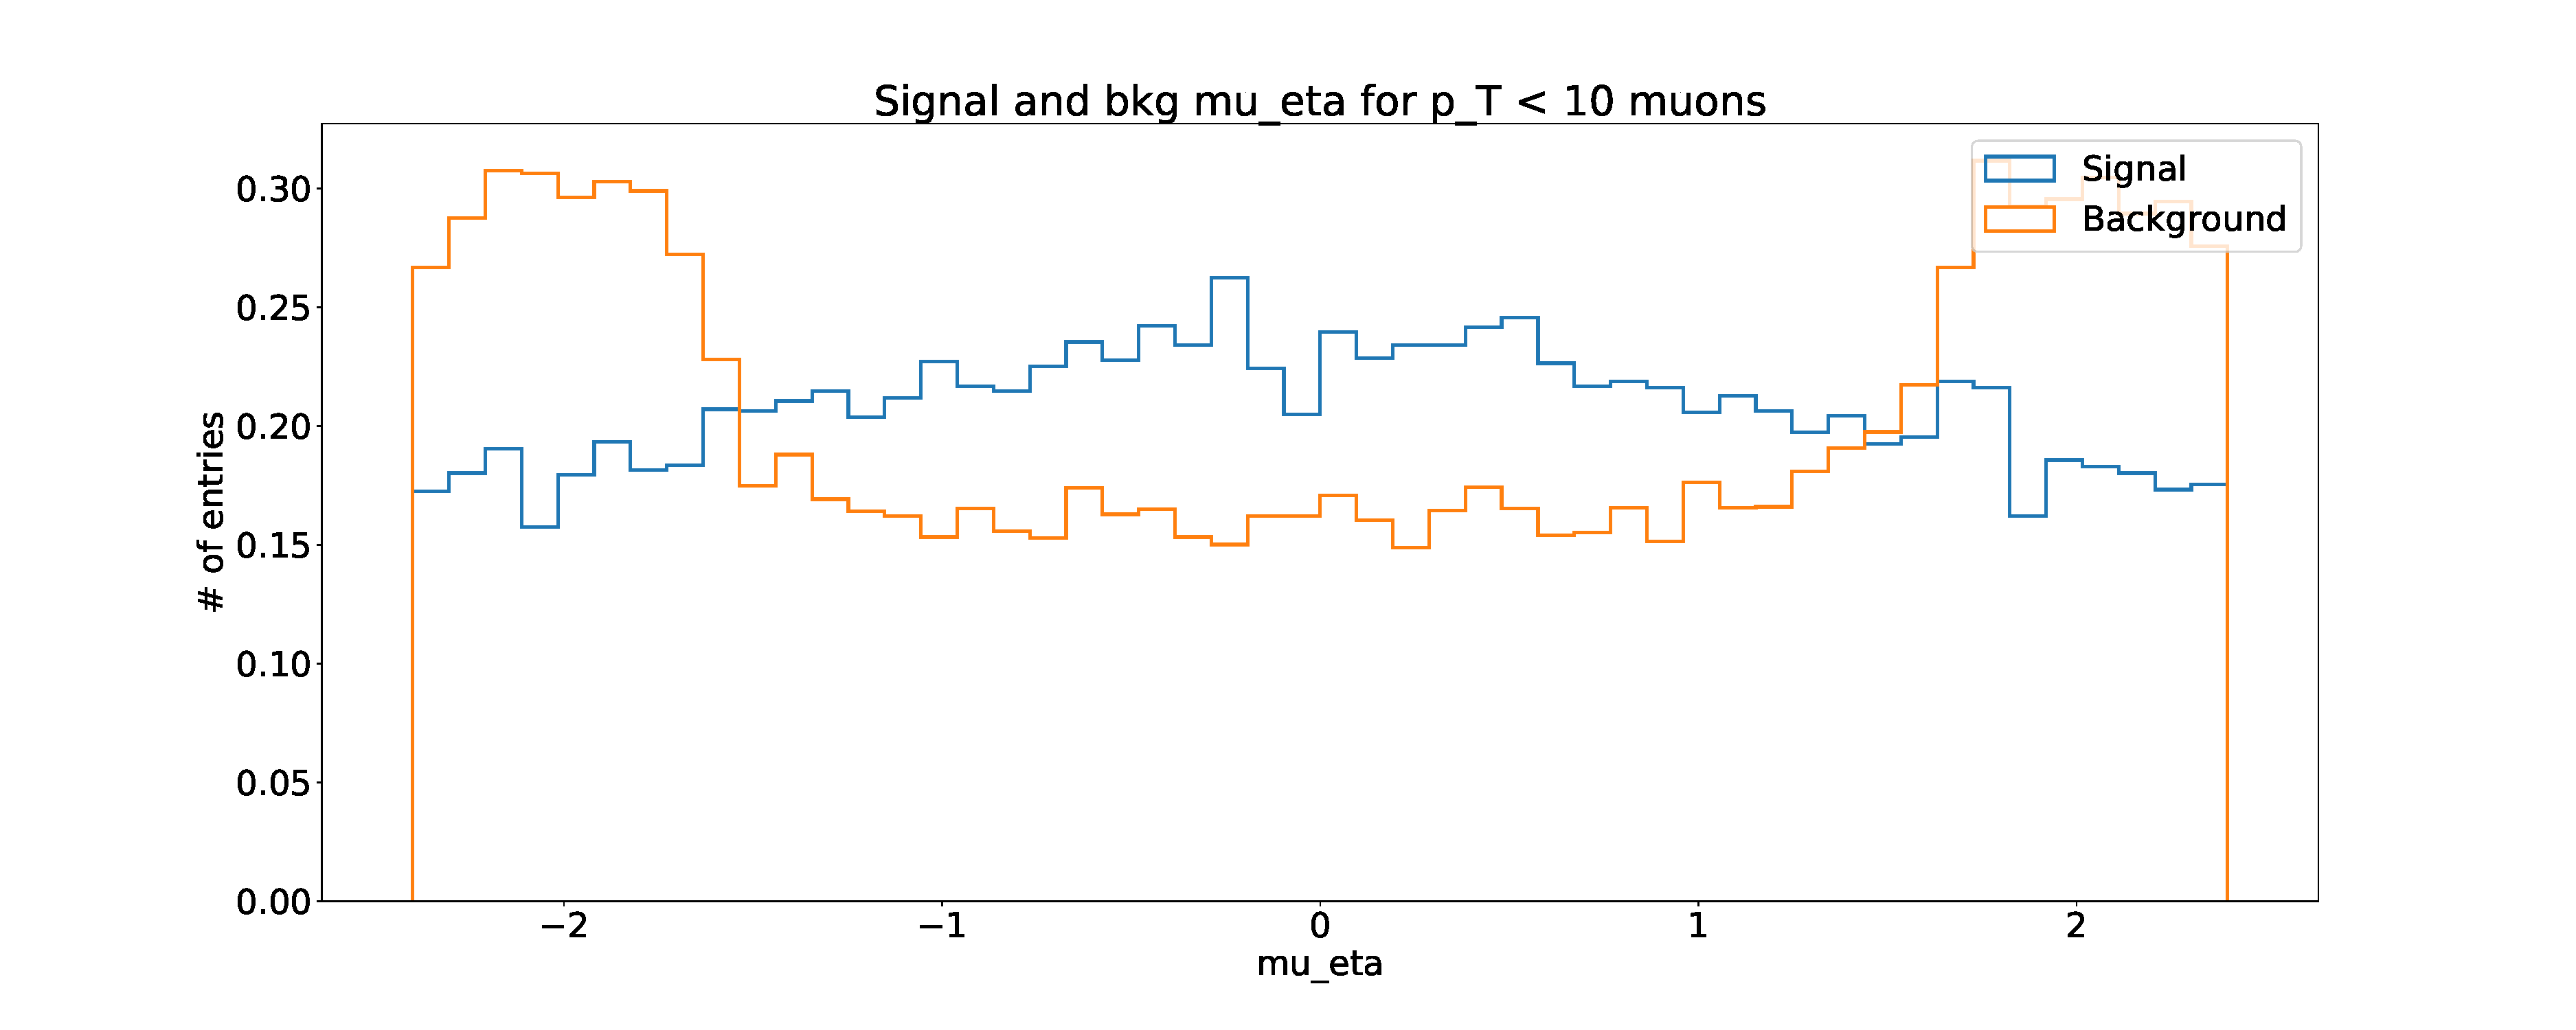
\includegraphics[width=0.45\textwidth]{Figures/Muons/mu_eta_5.pdf}
      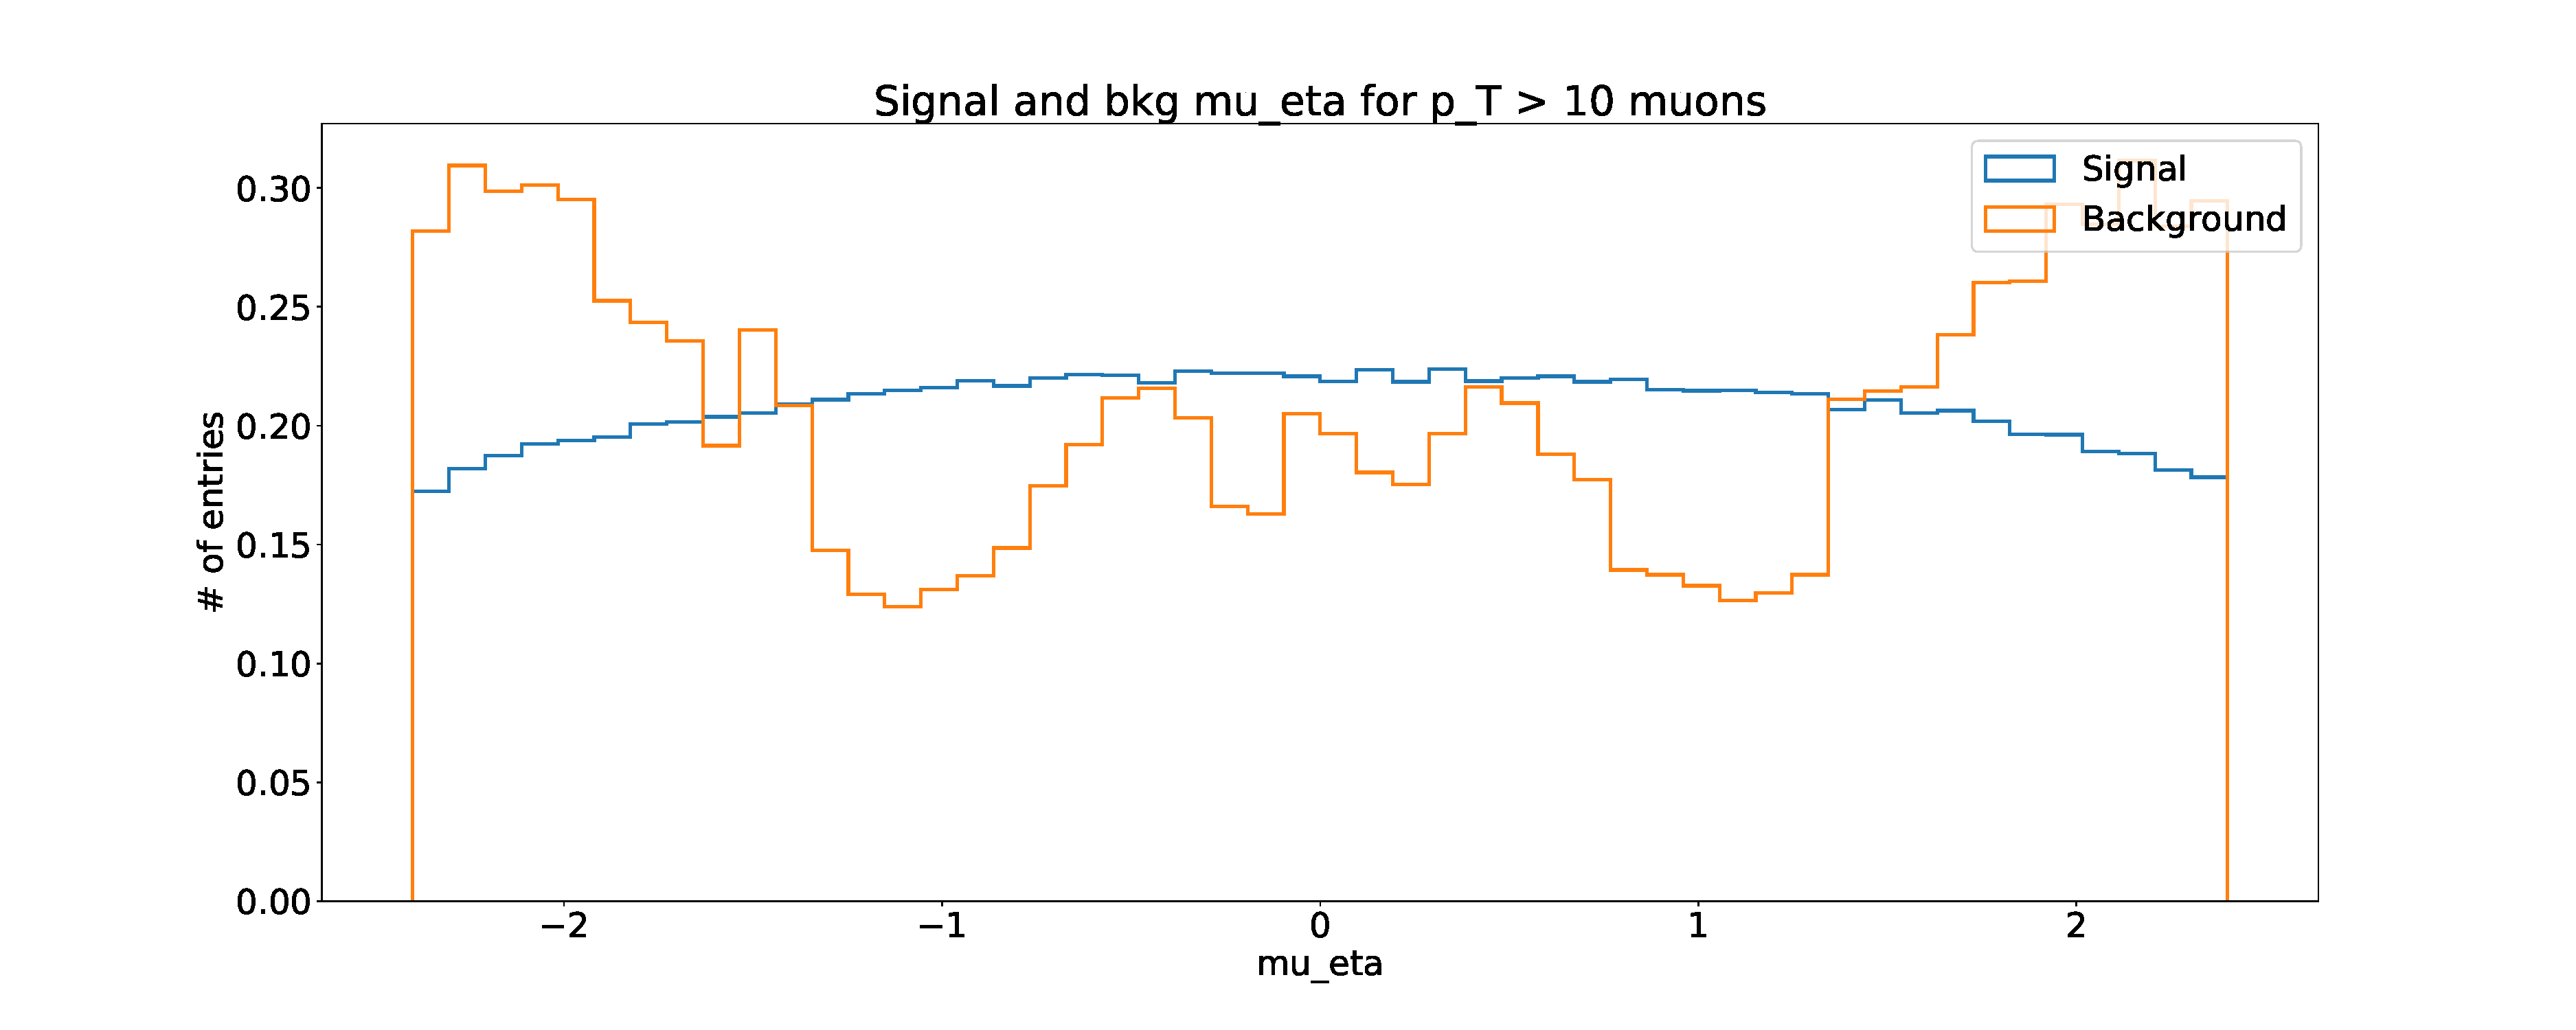
\includegraphics[width=0.45\textwidth]{Figures/Muons/mu_eta_10.pdf} \\
      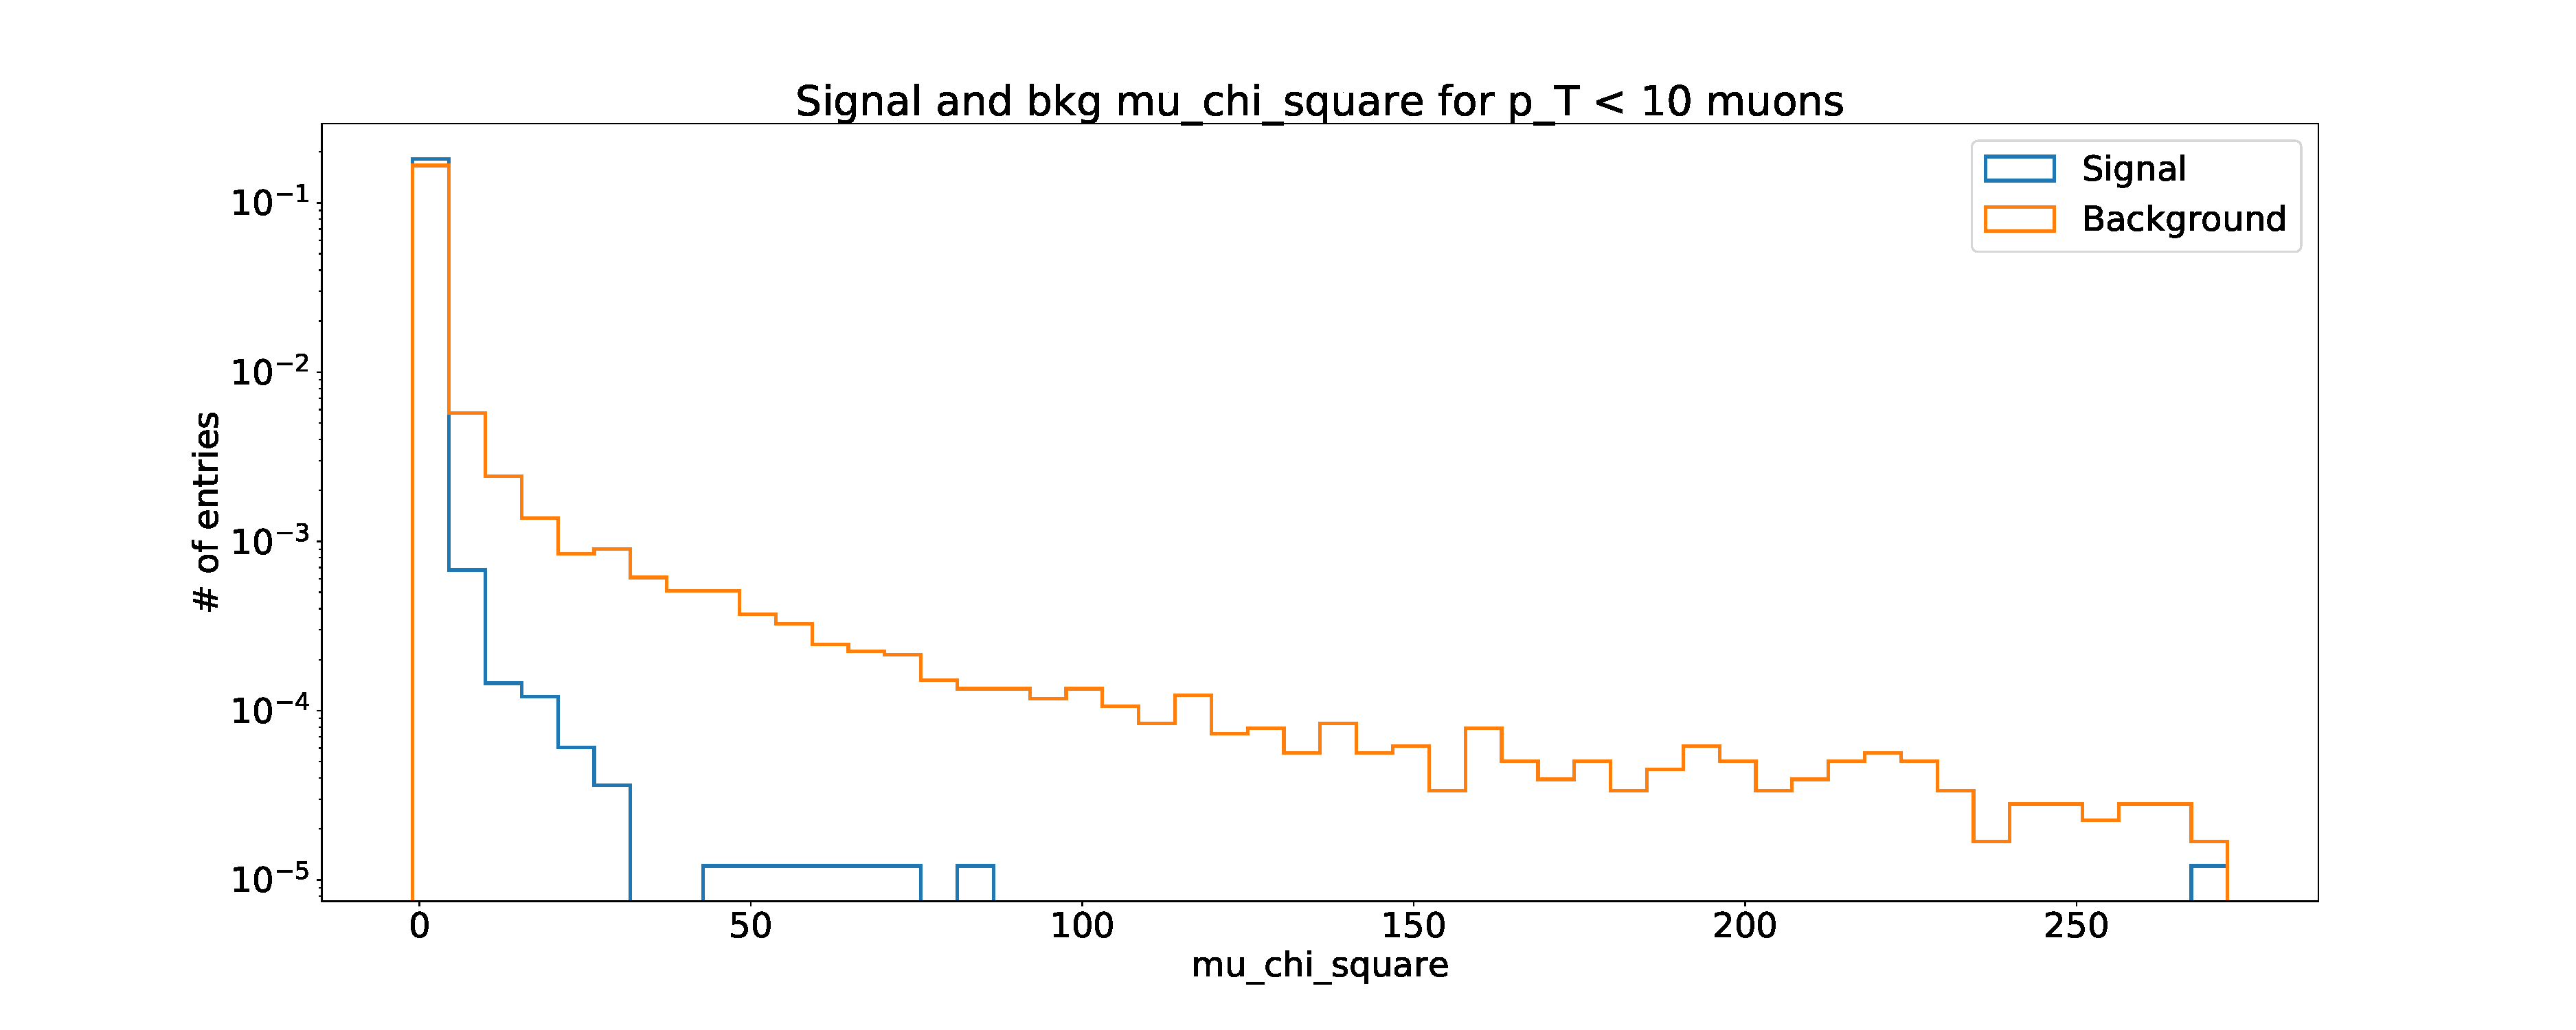
\includegraphics[width=0.45\textwidth]{Figures/Muons/mu_chi_square_5.pdf}
      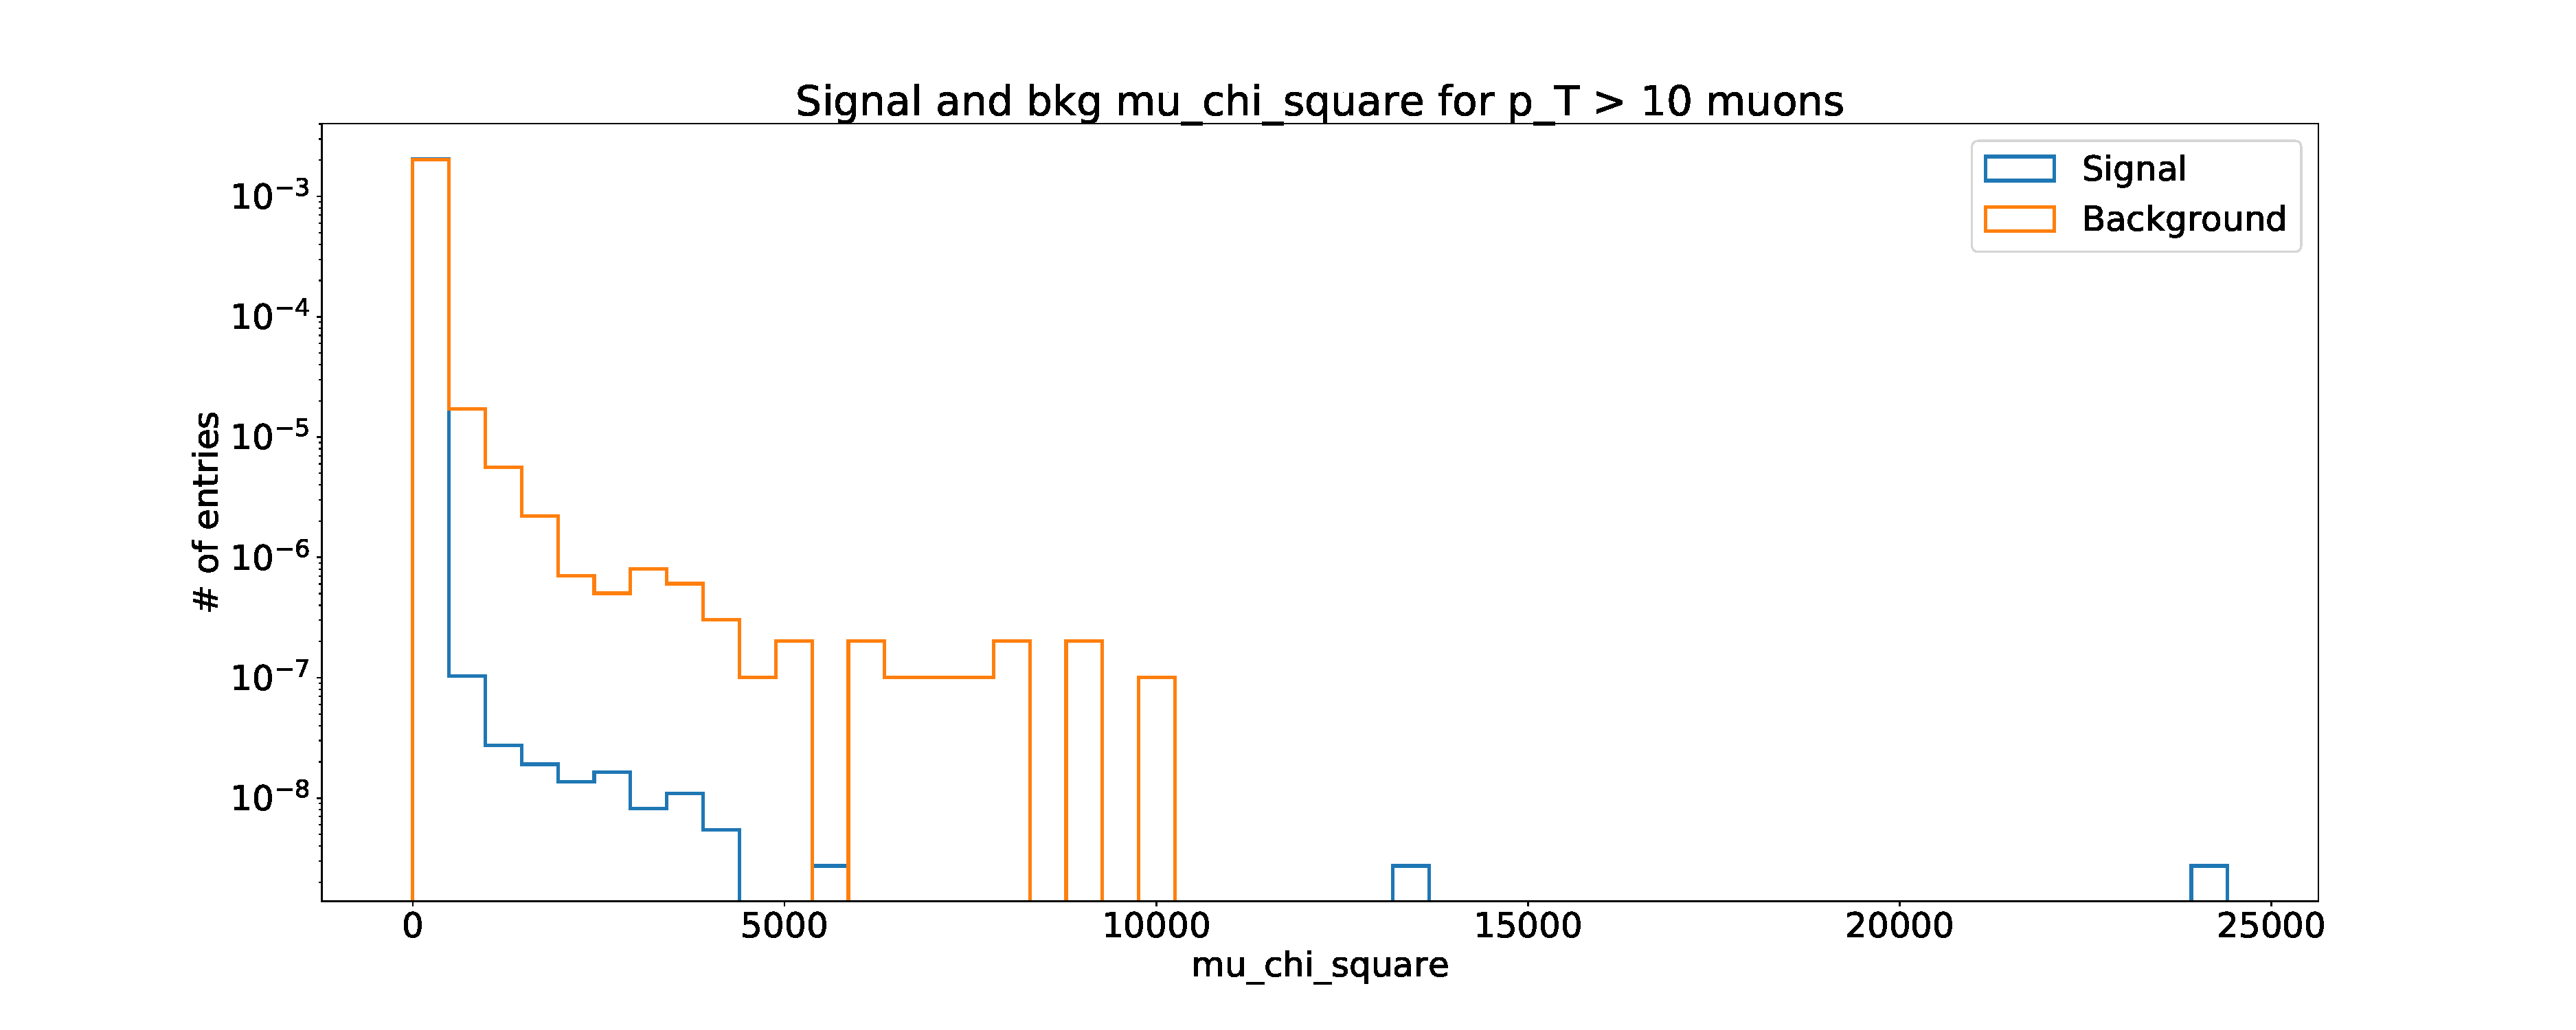
\includegraphics[width=0.45\textwidth]{Figures/Muons/mu_chi_square_10.pdf} \\
      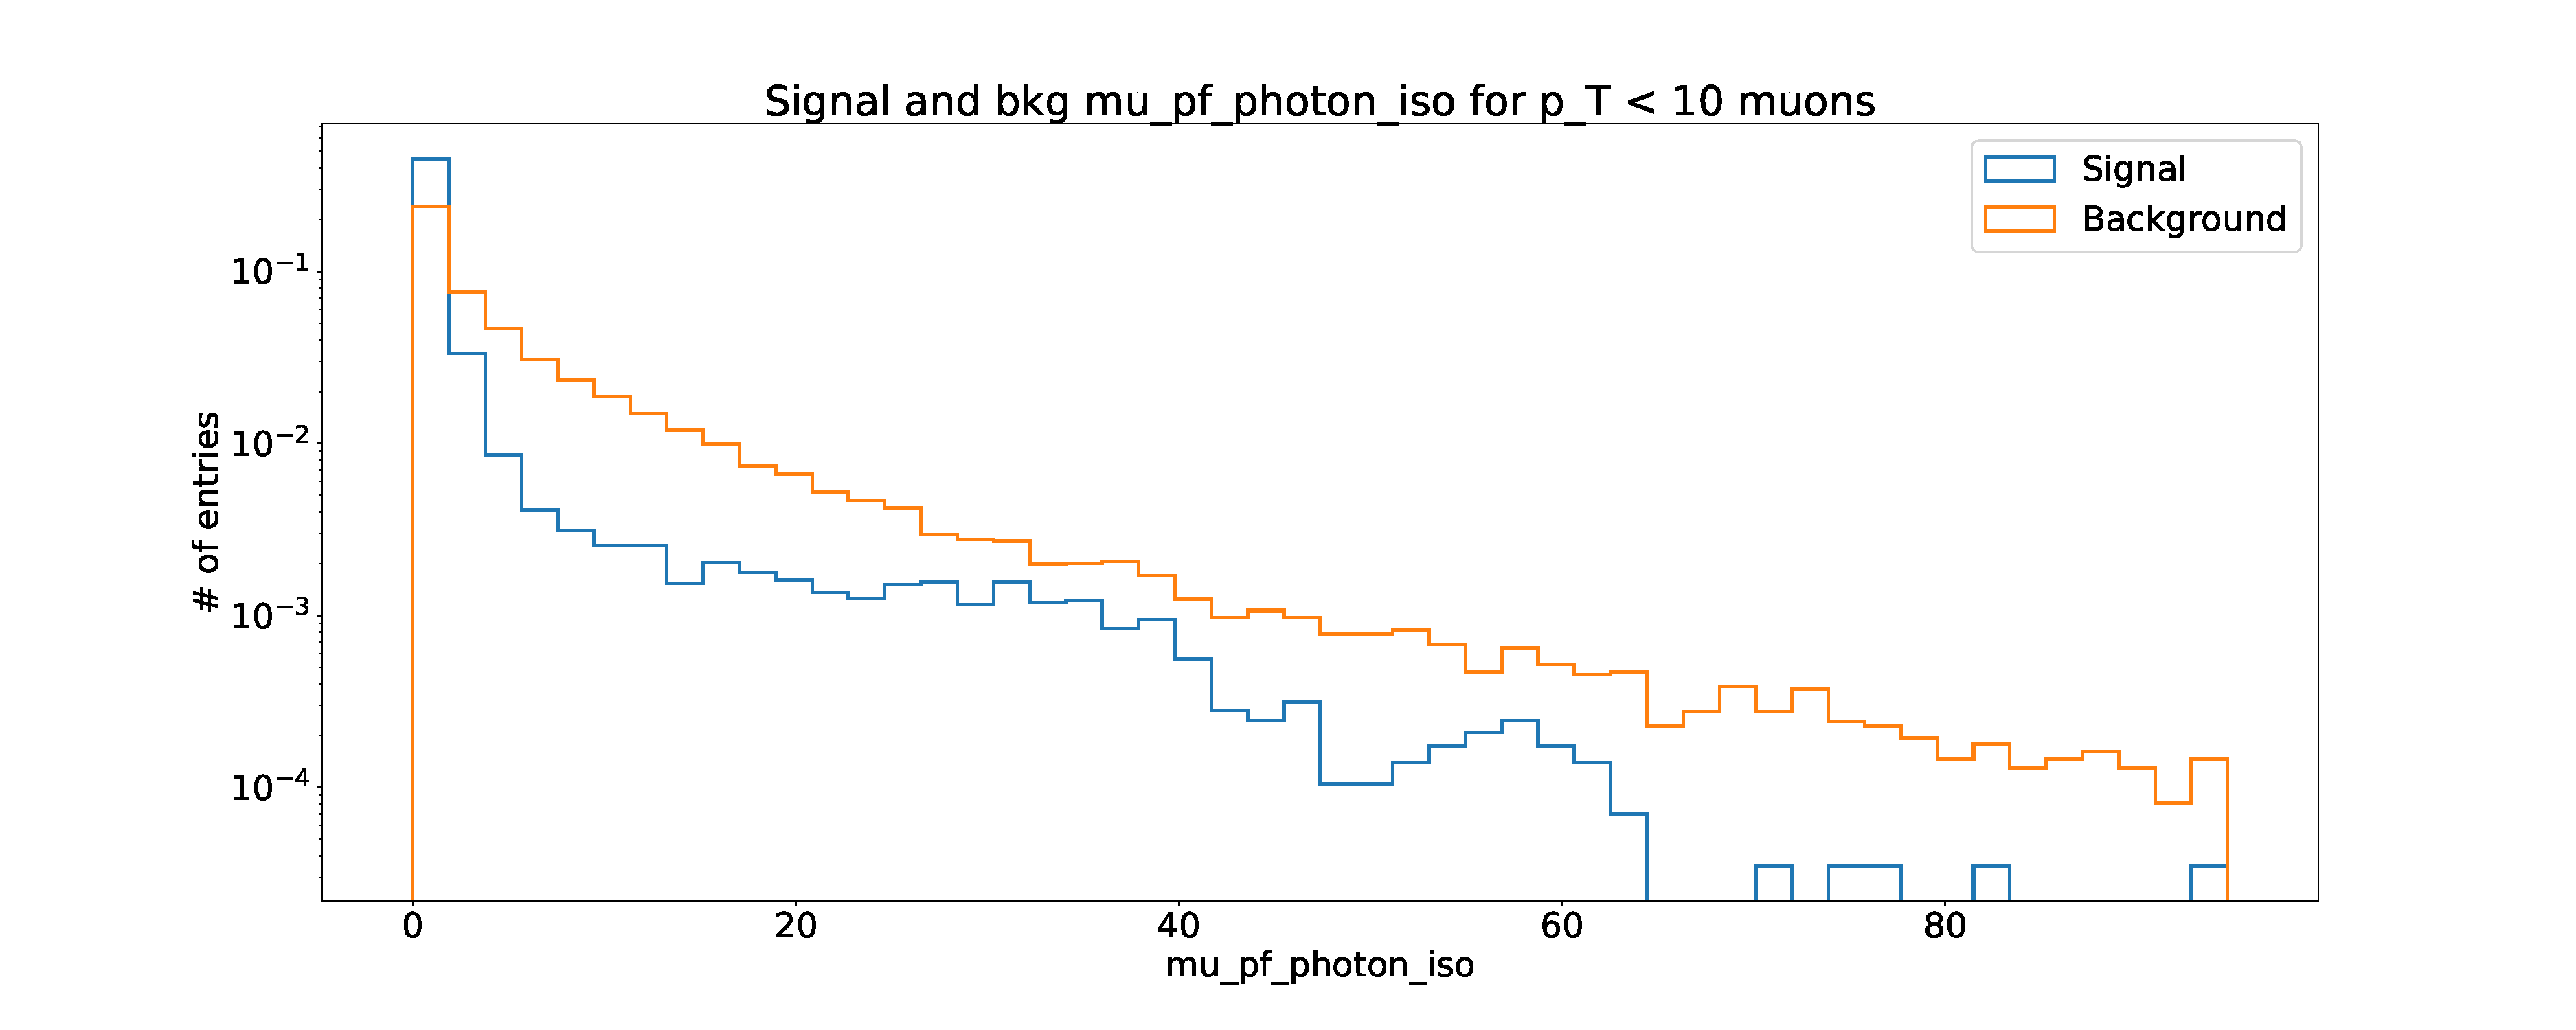
\includegraphics[width=0.45\textwidth]{Figures/Muons/mu_pf_photon_iso_5.pdf}
      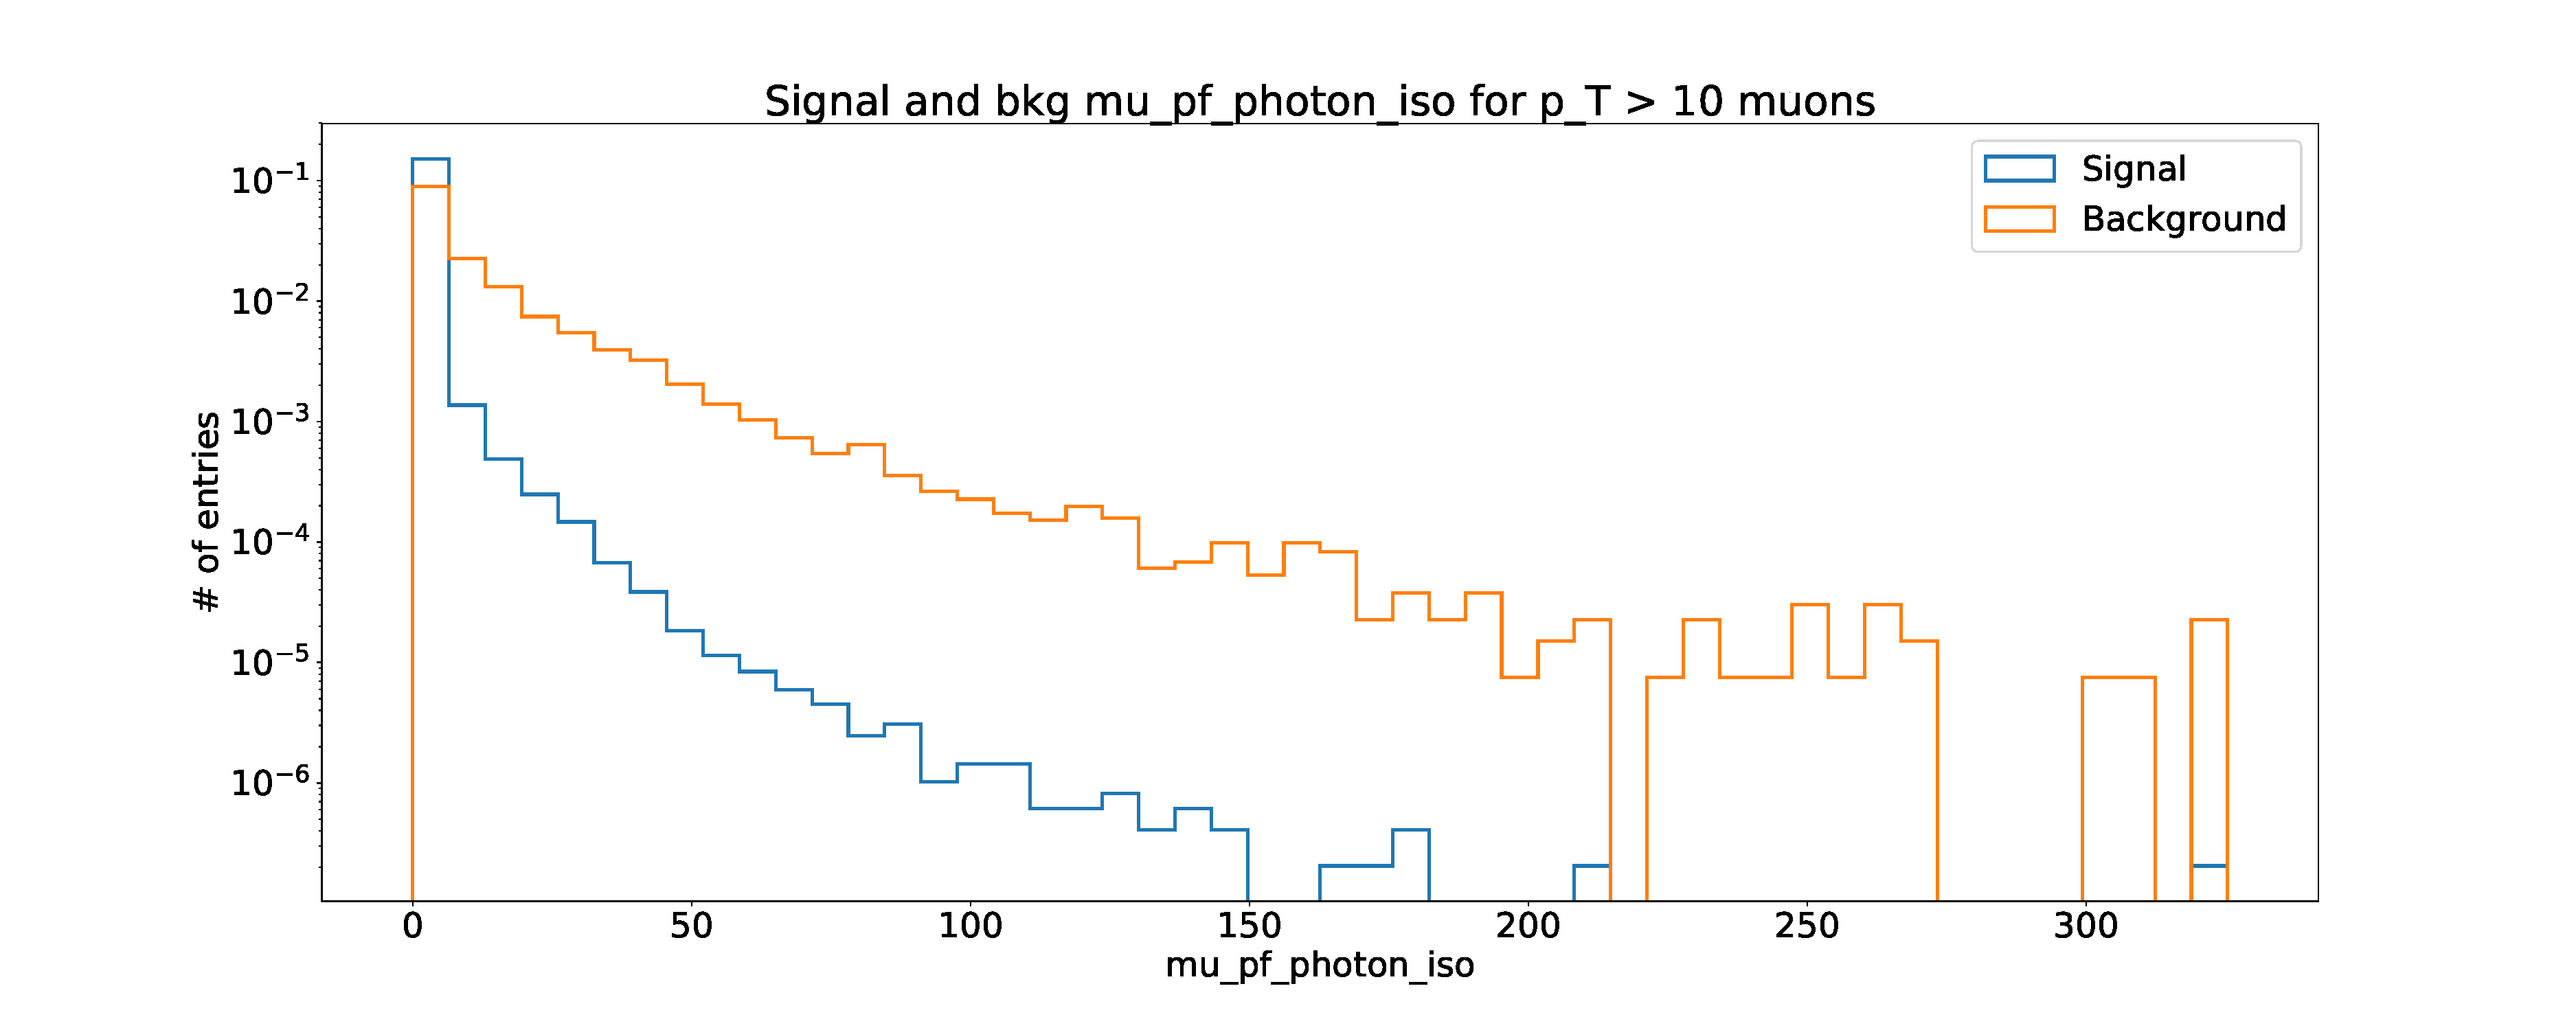
\includegraphics[width=0.45\textwidth]{Figures/Muons/mu_pf_photon_iso_10.pdf} \\
      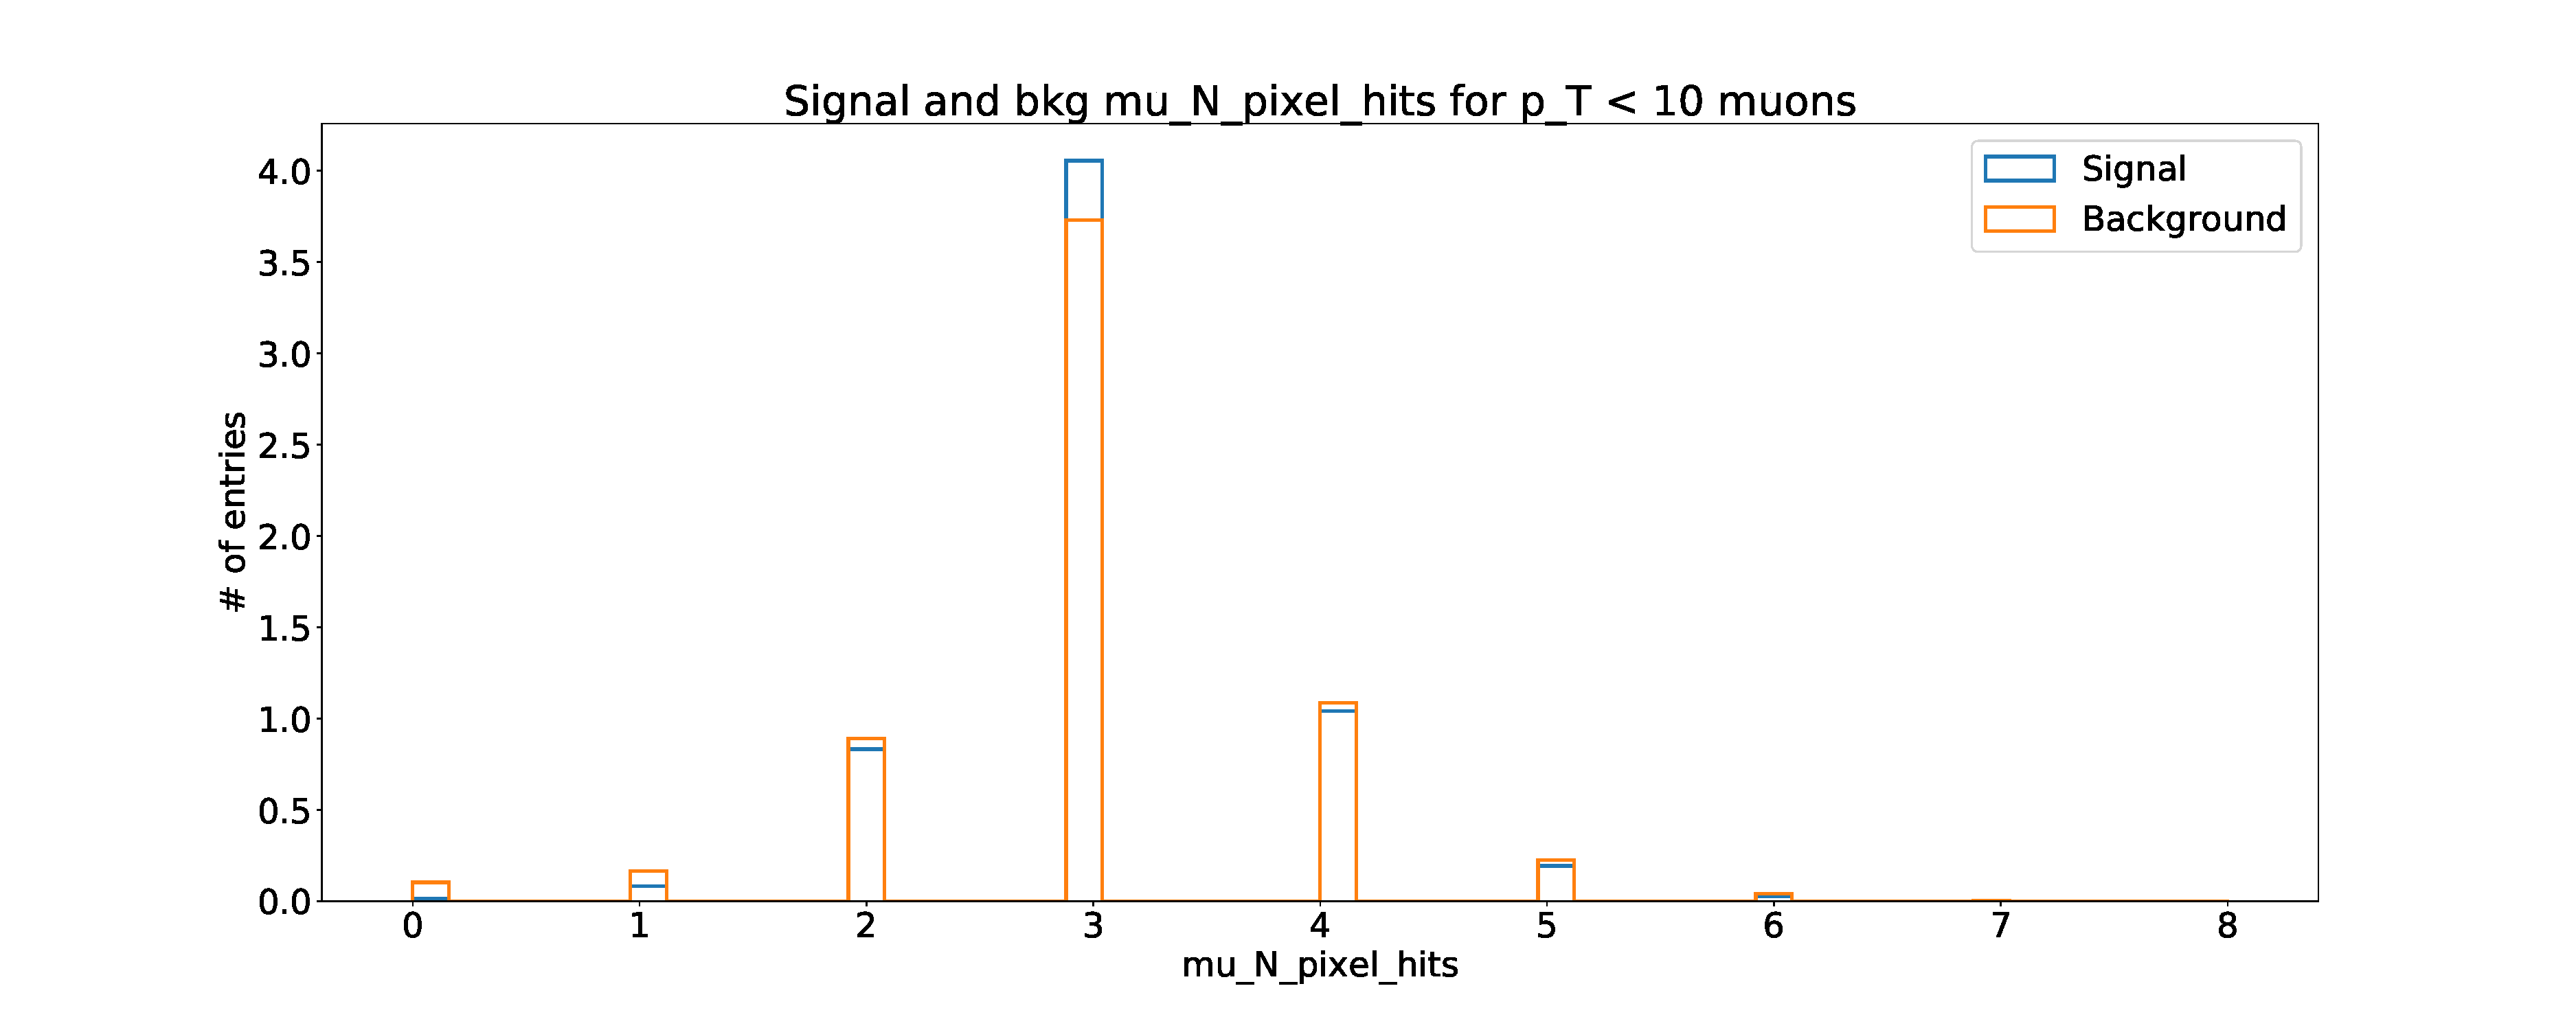
\includegraphics[width=0.45\textwidth]{Figures/Muons/mu_N_pixel_hits_5.pdf}
      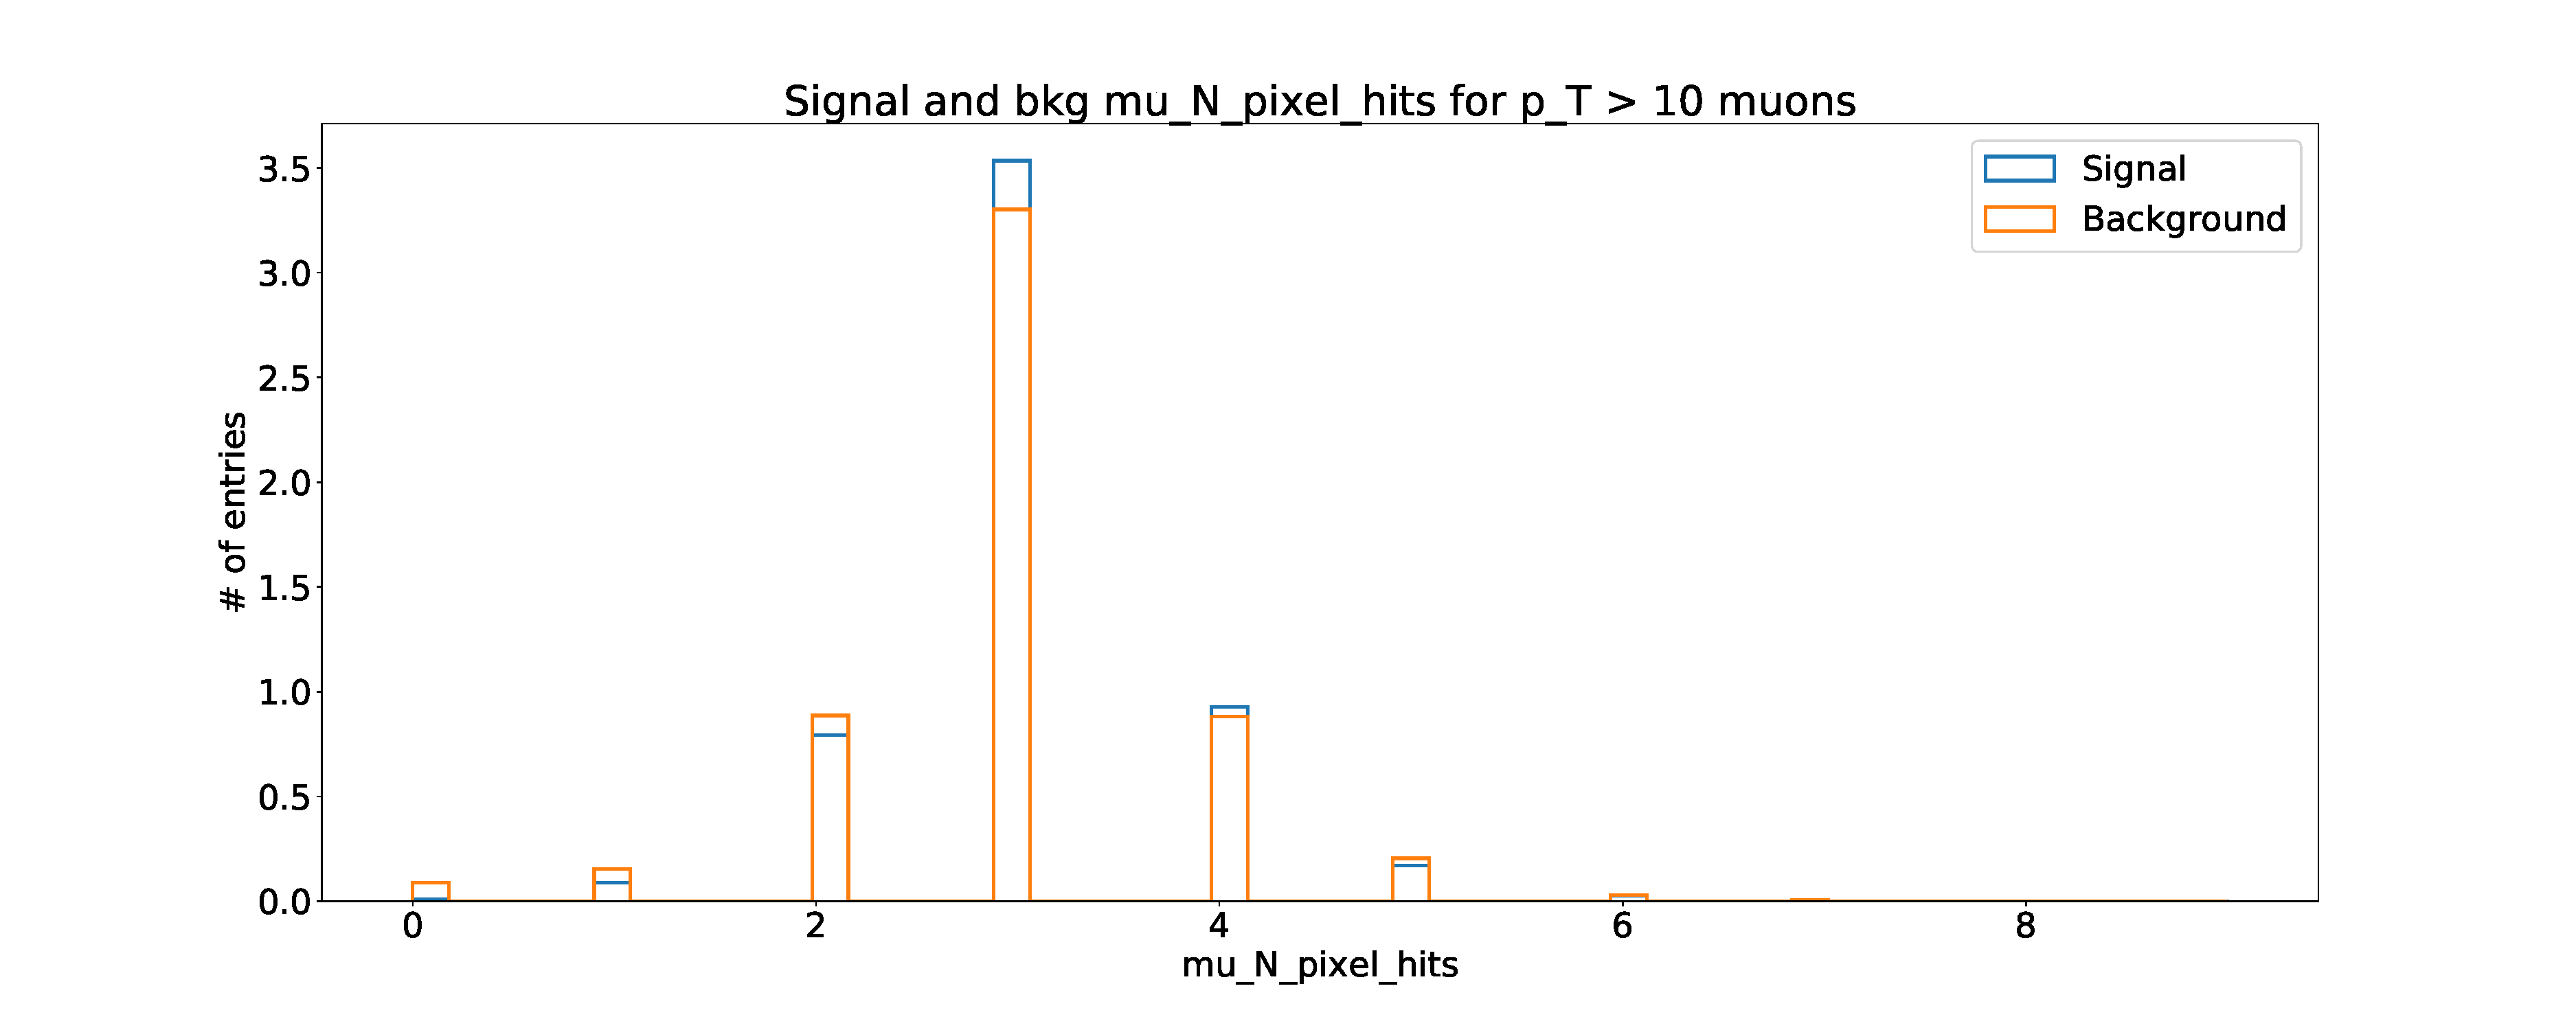
\includegraphics[width=0.45\textwidth]{Figures/Muons/mu_N_pixel_hits_10.pdf} \\
   \caption{Distributions of some features used as the input for the MVA training on 2016 Drell-Yan with jets MC sample. Distributions are shown for muons with
   $5 < p_T < 10 $ GeV (left) and $p_T > 10$ GeV (right).}
   \label{fig:mu_features_2016}}
   \end{center}
\end{figure}

The working point (WP) is choosen as follows: yields of 3 main processes in the signal region are calculated using different WPs for different Muon MVA signal
efficiencies:

\begin{itemize}
   \item Low $p_T$ scanned in steps of 5\% (75\% - 95\%), high $p_T$ in steps of 1\% (95\% - 99\%).
   \item Our previous PF muon ID + RelPFiso + SIP3D efficiency was 75\% - 95\%.
   \item Z+X estimated using SS method only with recalculated Fake Rates for each WP.
   \item Plot $S/\sqrt(S+B)$ in search for the optimal WP choice.
\end{itemize}

The MVA score distribution together with the Working Point choice is shown in the Fig.~\ref{fig:mu_MVA_score_2016} for 2016, Fig.~\ref{fig:mu_MVA_score_2017}
for 2017, and Fig.~\ref{fig:mu_MVA_score_2018} for 2018 data taking periods.

\begin{figure}[!htb]
   \vspace*{0.3cm}
   \begin{center}
      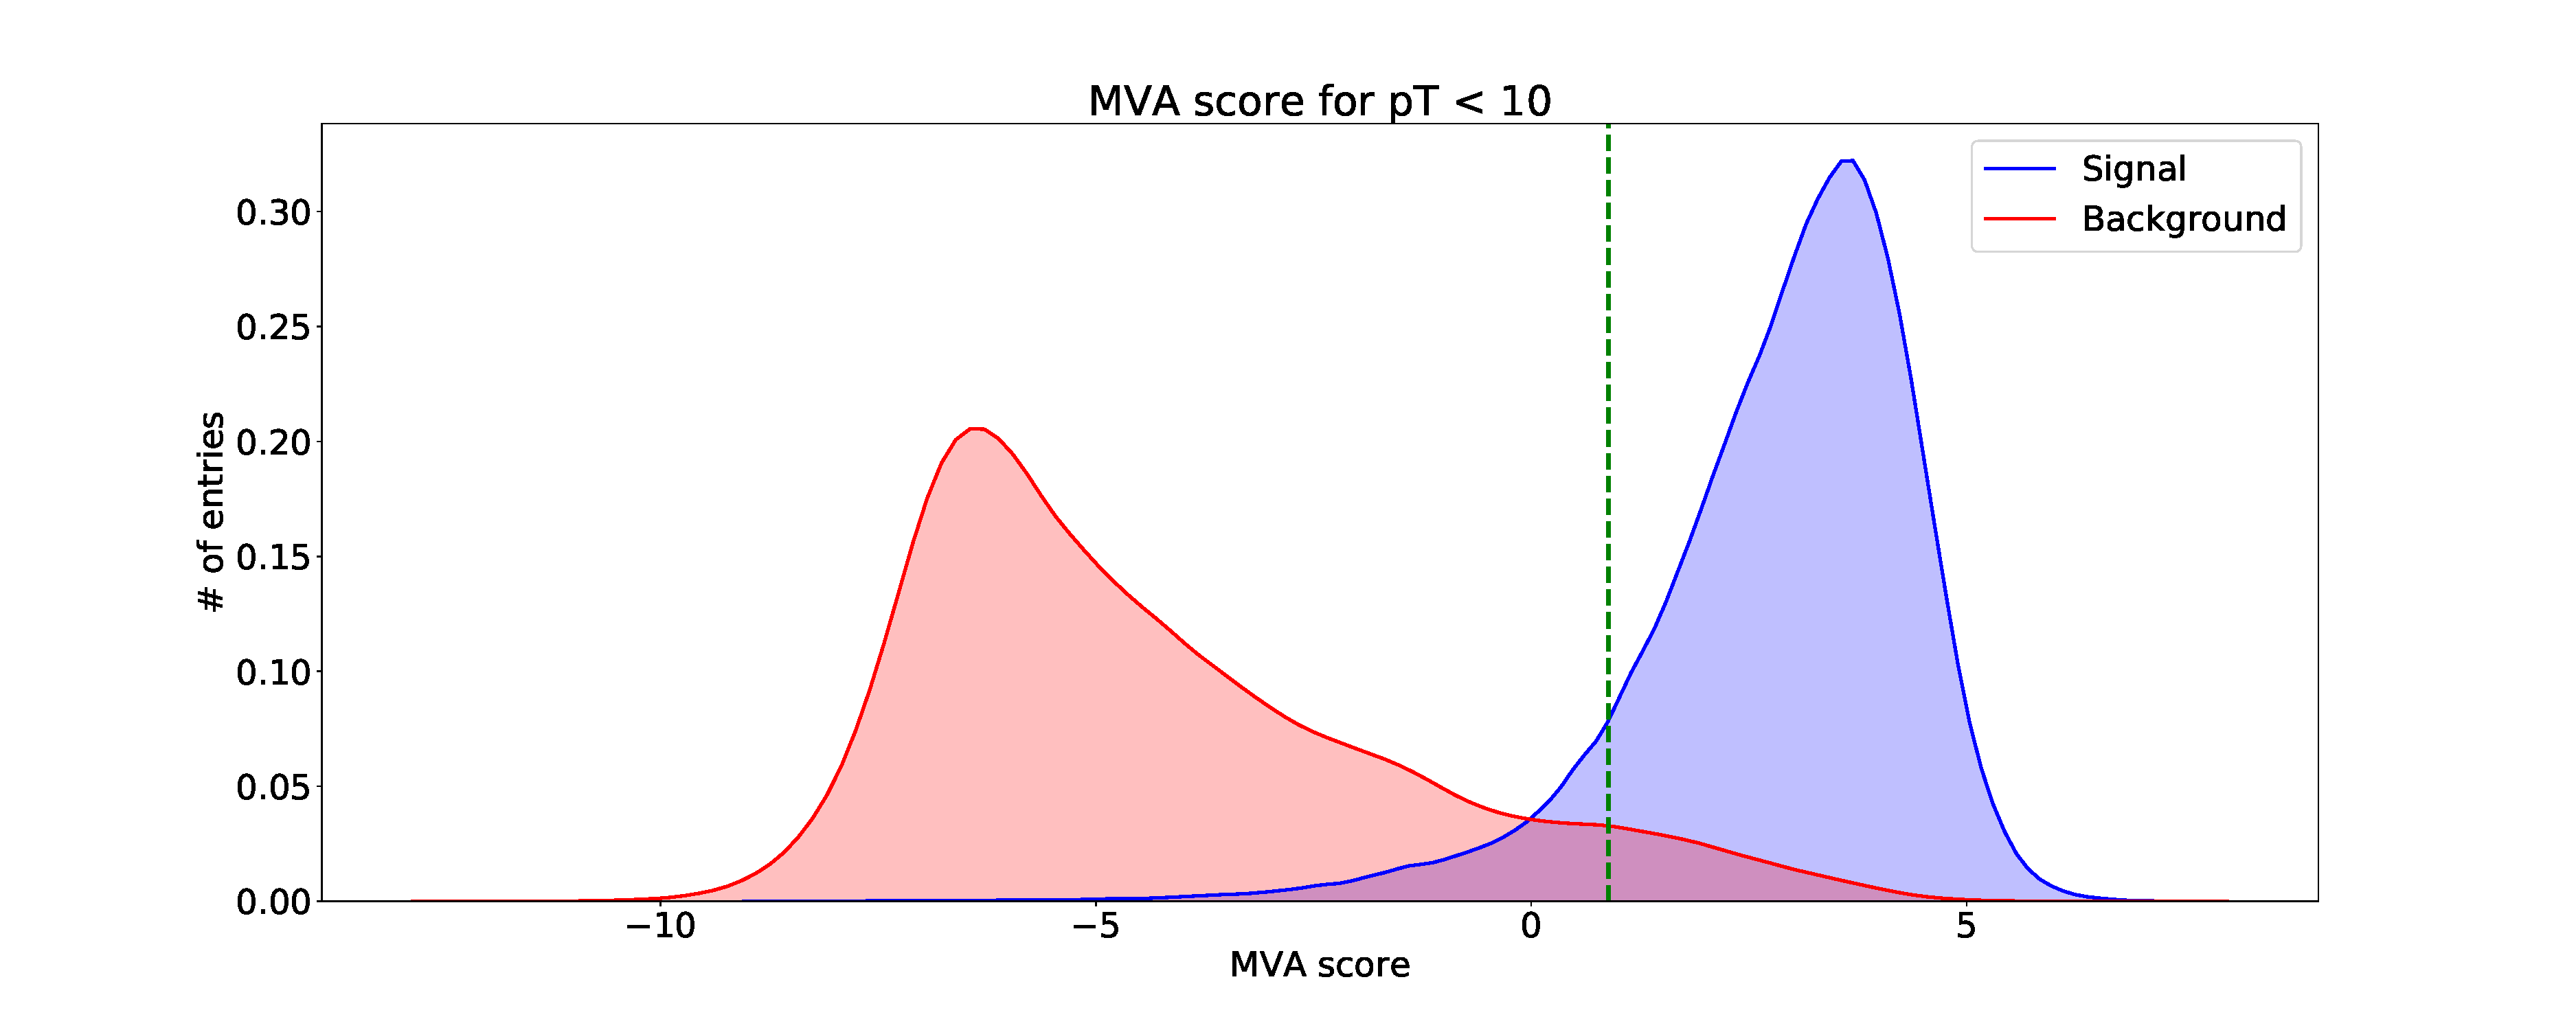
\includegraphics[width=0.95\textwidth]{Figures/Muons/MVA_score_5_2016.pdf}\\
      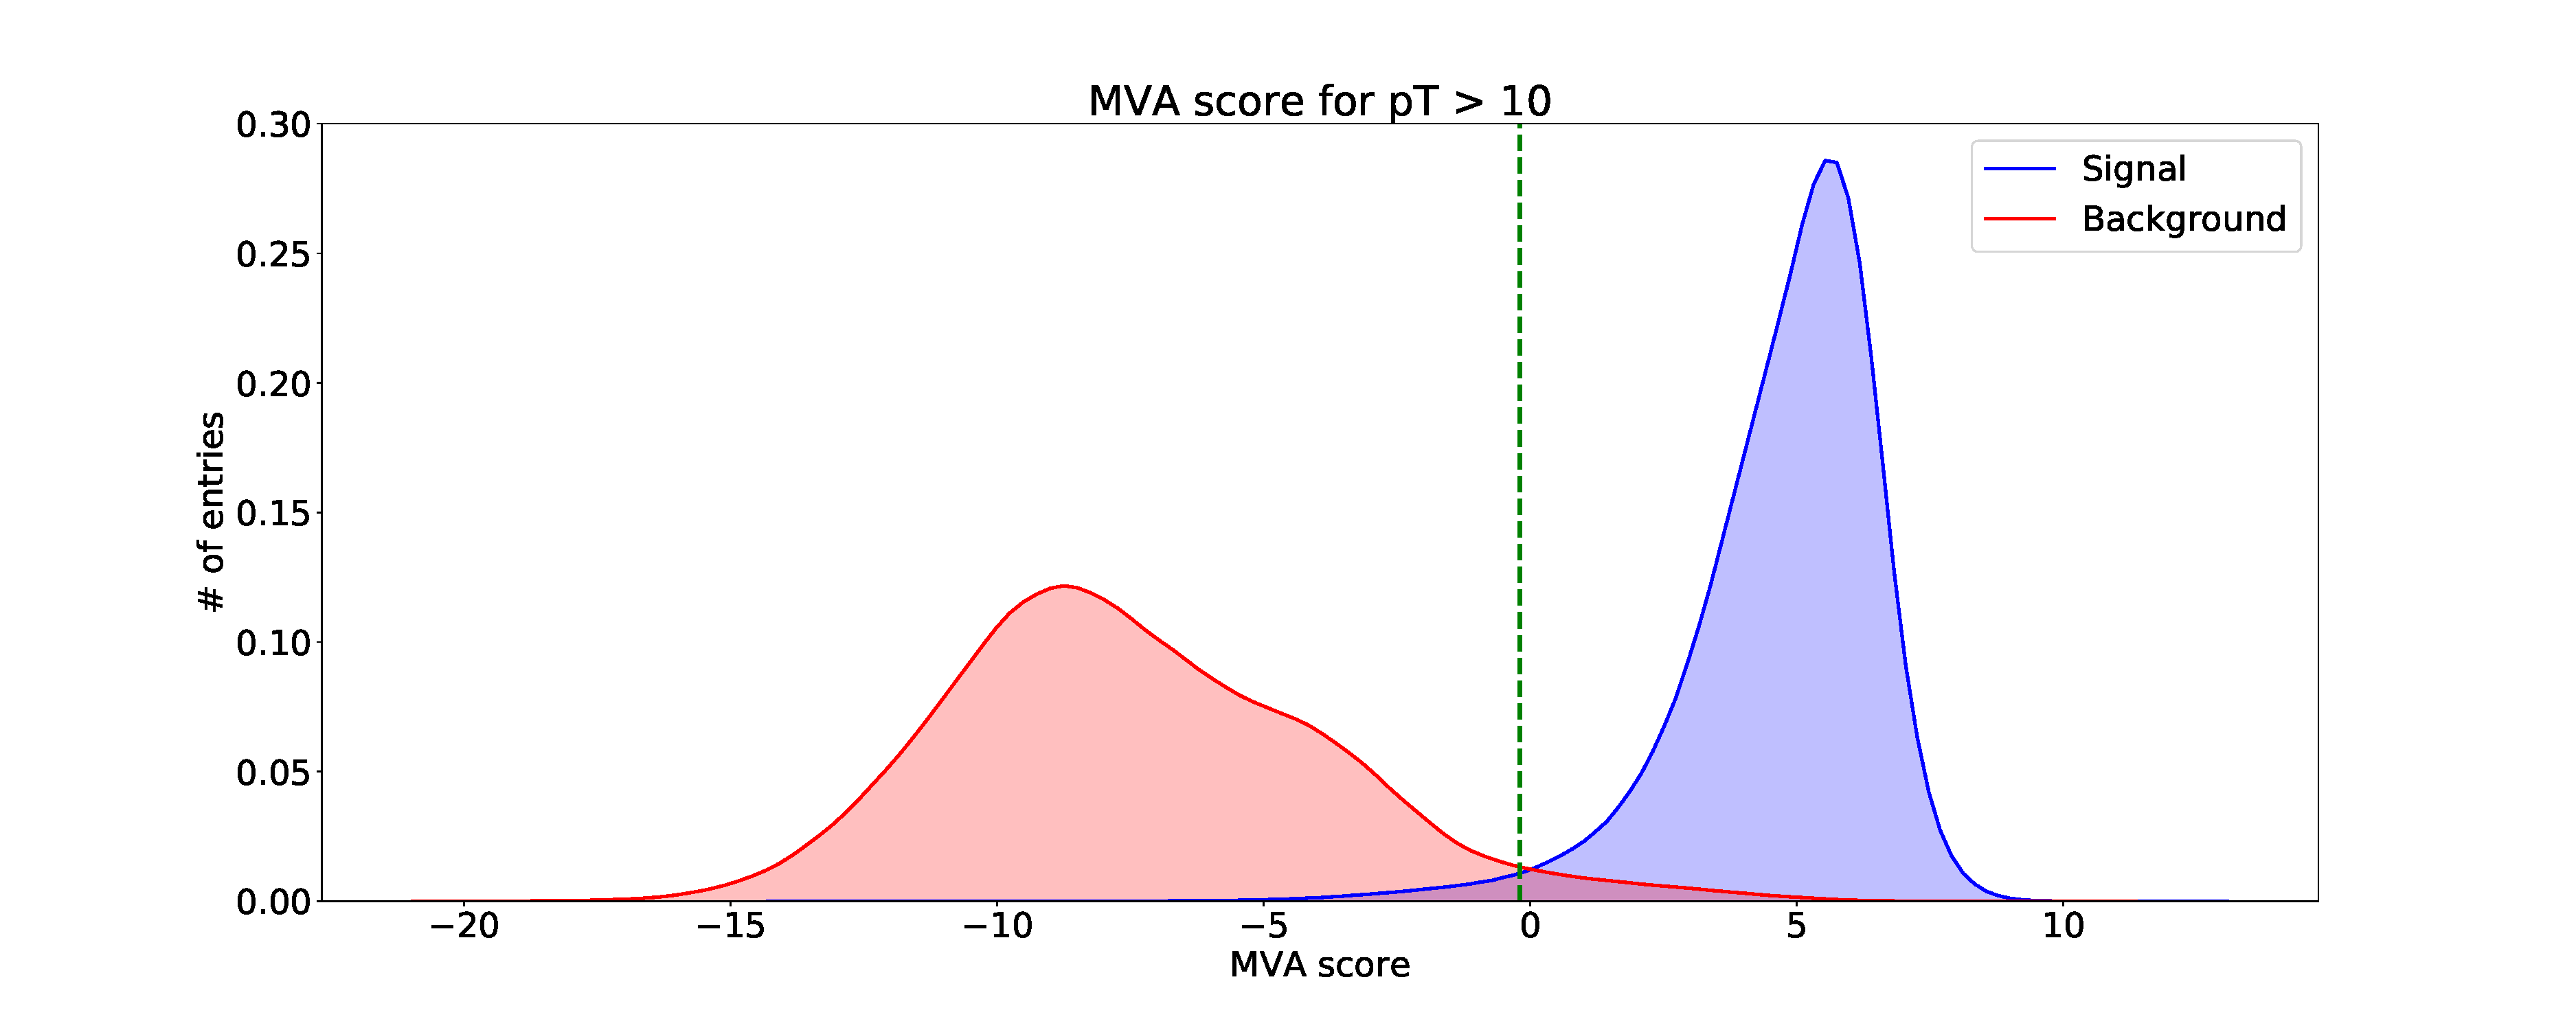
\includegraphics[width=0.95\textwidth]{Figures/Muons/MVA_score_10_2016.pdf}
   \caption{The MVA score and Working Point choice for the MVA trained on 2016 Drell-Yan with jets MC sample. The MVA score is shown for muons with
   $5 < p_T < 10 $ GeV (top) and $p_T > 10$ GeV (bottom).}
   \label{fig:mu_MVA_score_2017}
   \end{center}
\end{figure}

\begin{figure}[!htb]
   \vspace*{0.3cm}
   \begin{center}
      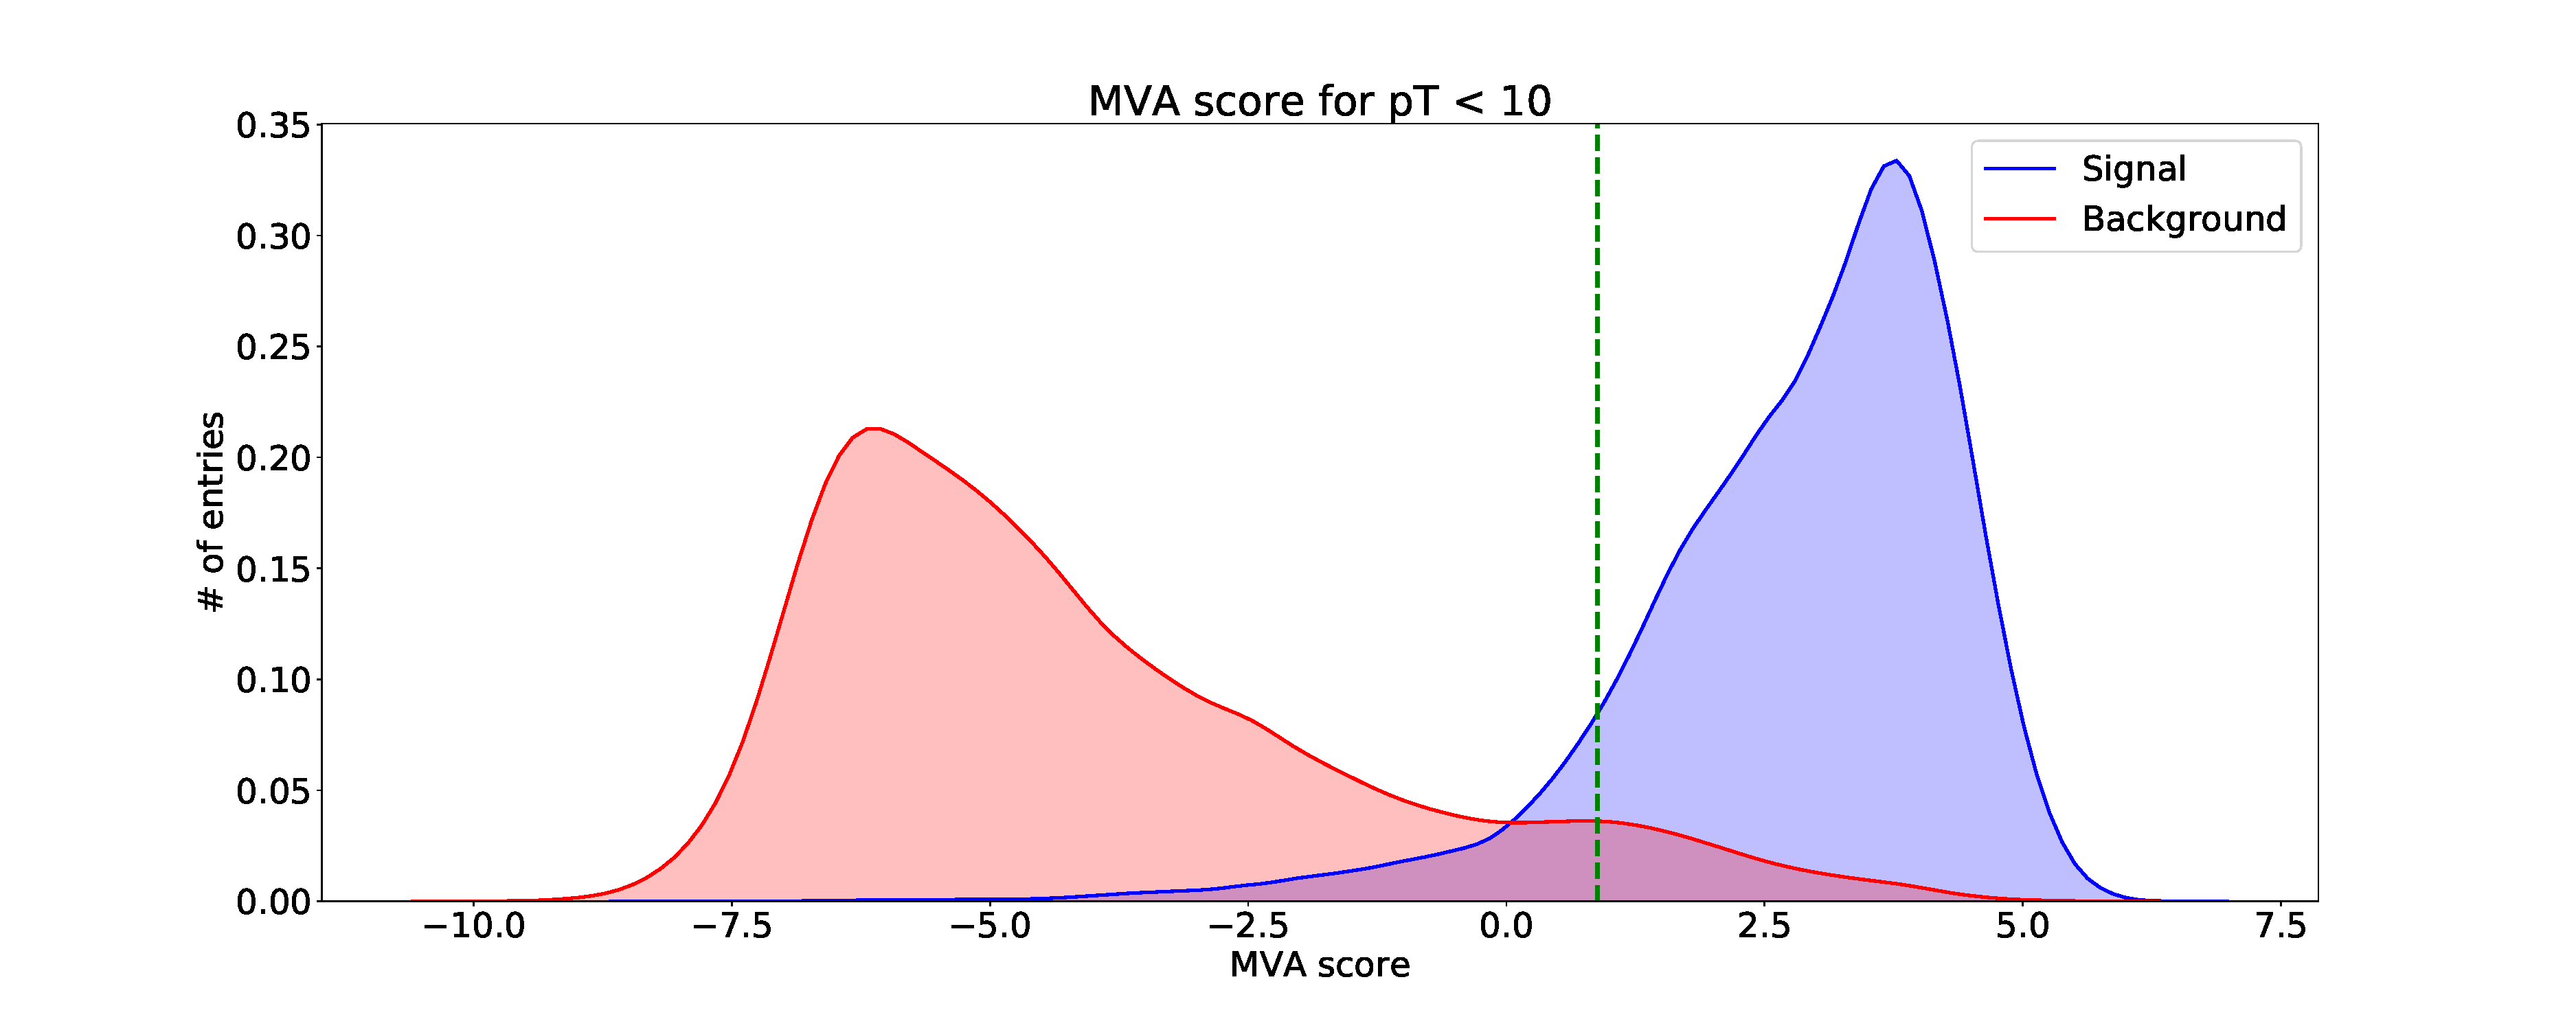
\includegraphics[width=0.95\textwidth]{Figures/Muons/MVA_score_5_2017.pdf}\\
      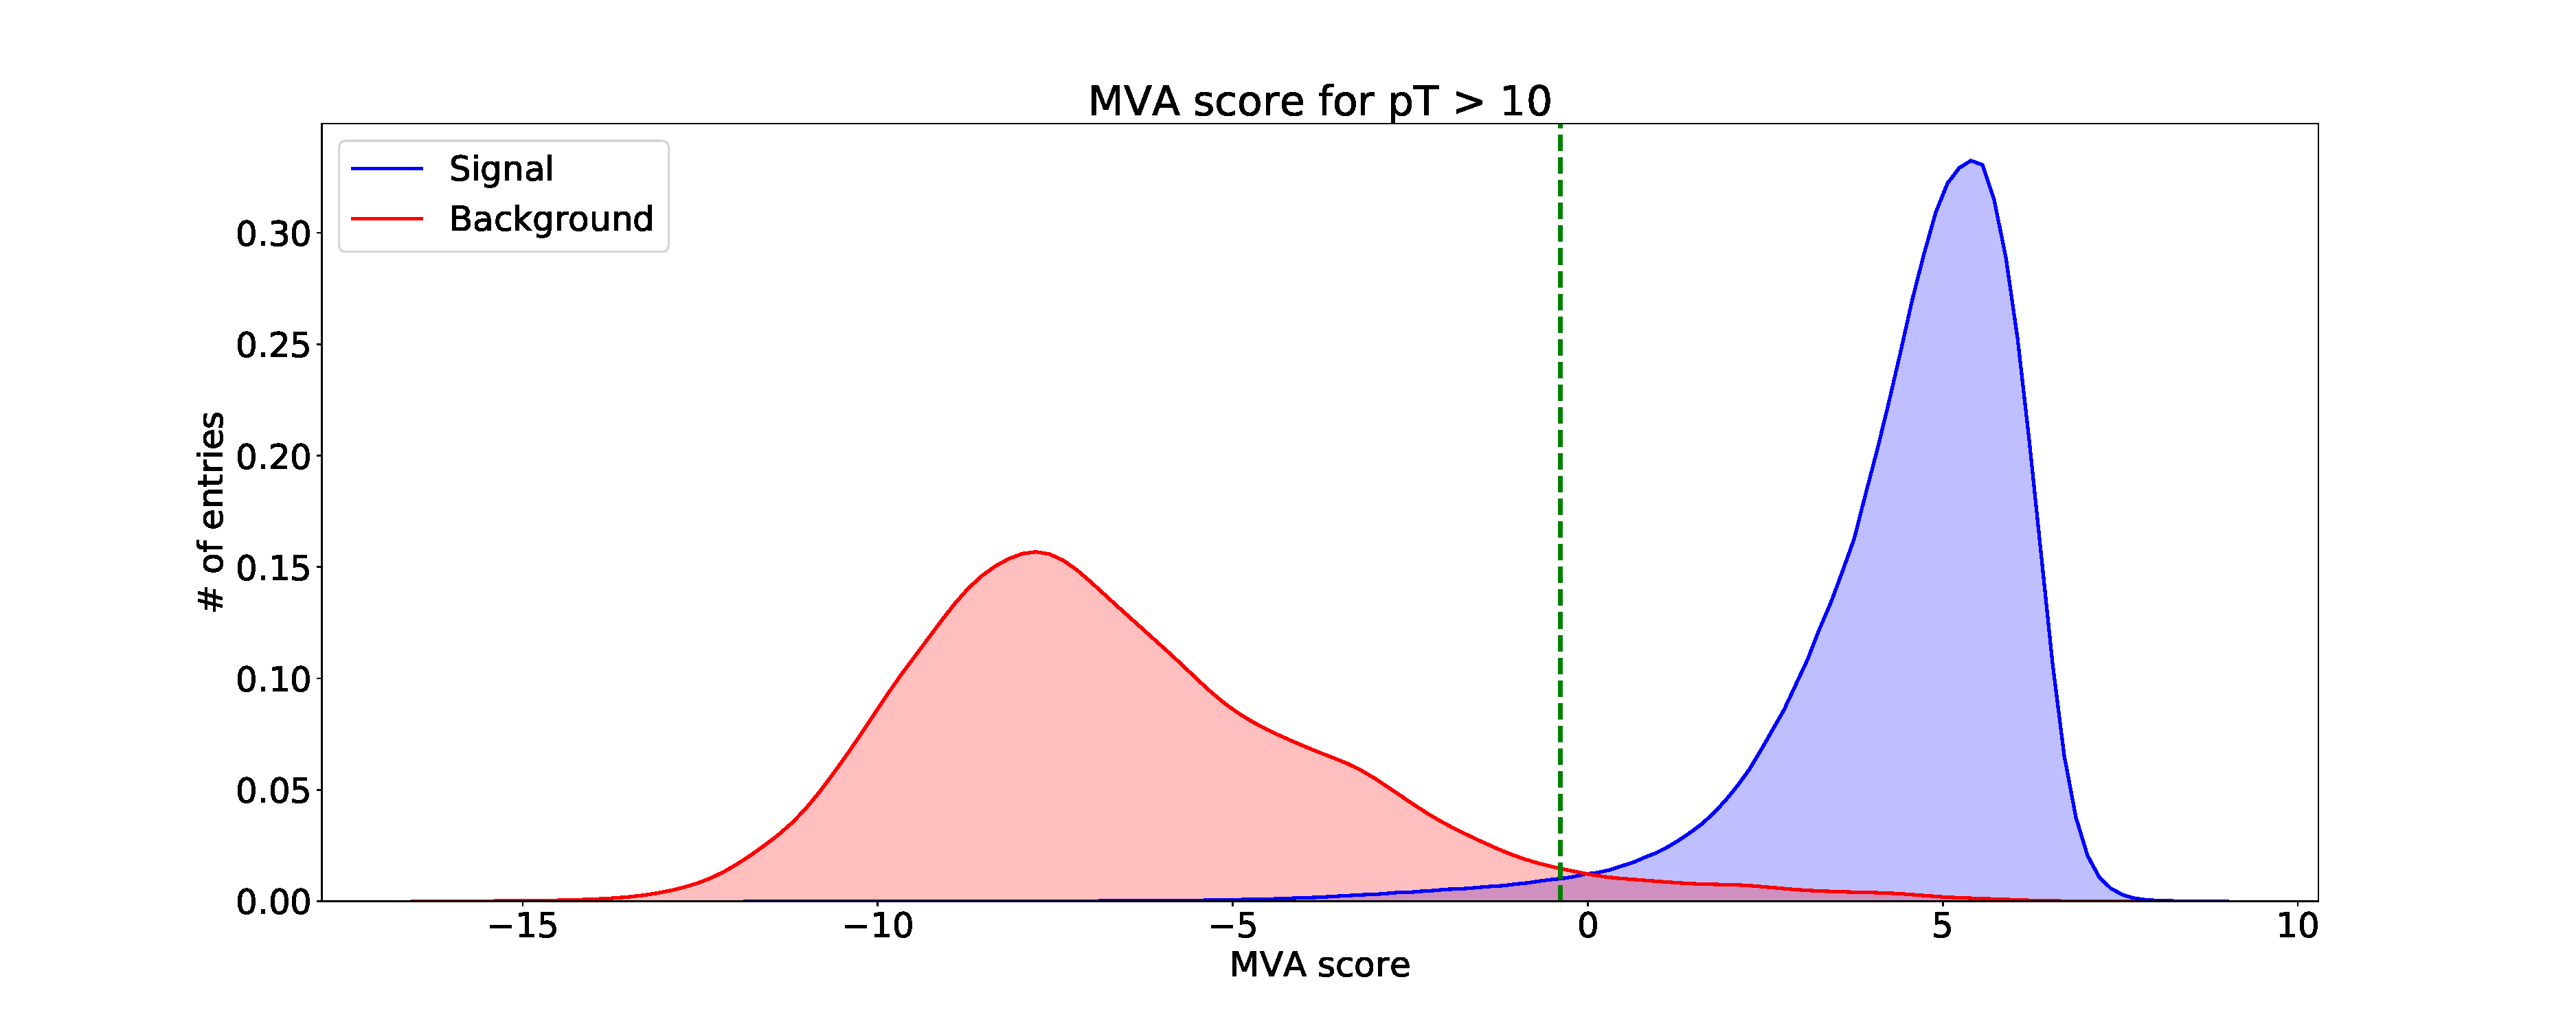
\includegraphics[width=0.95\textwidth]{Figures/Muons/MVA_score_10_2017.pdf}
   \caption{The MVA score and Working Point choice for the MVA trained on 2017 Drell-Yan with jets MC sample. The MVA score is shown for muons with
   $5 < p_T < 10 $ GeV (top) and $p_T > 10$ GeV (bottom).}
   \label{fig:mu_MVA_score_2017}
   \end{center}
\end{figure}

\begin{figure}[!htb]
   \vspace*{0.3cm}
   \begin{center}
      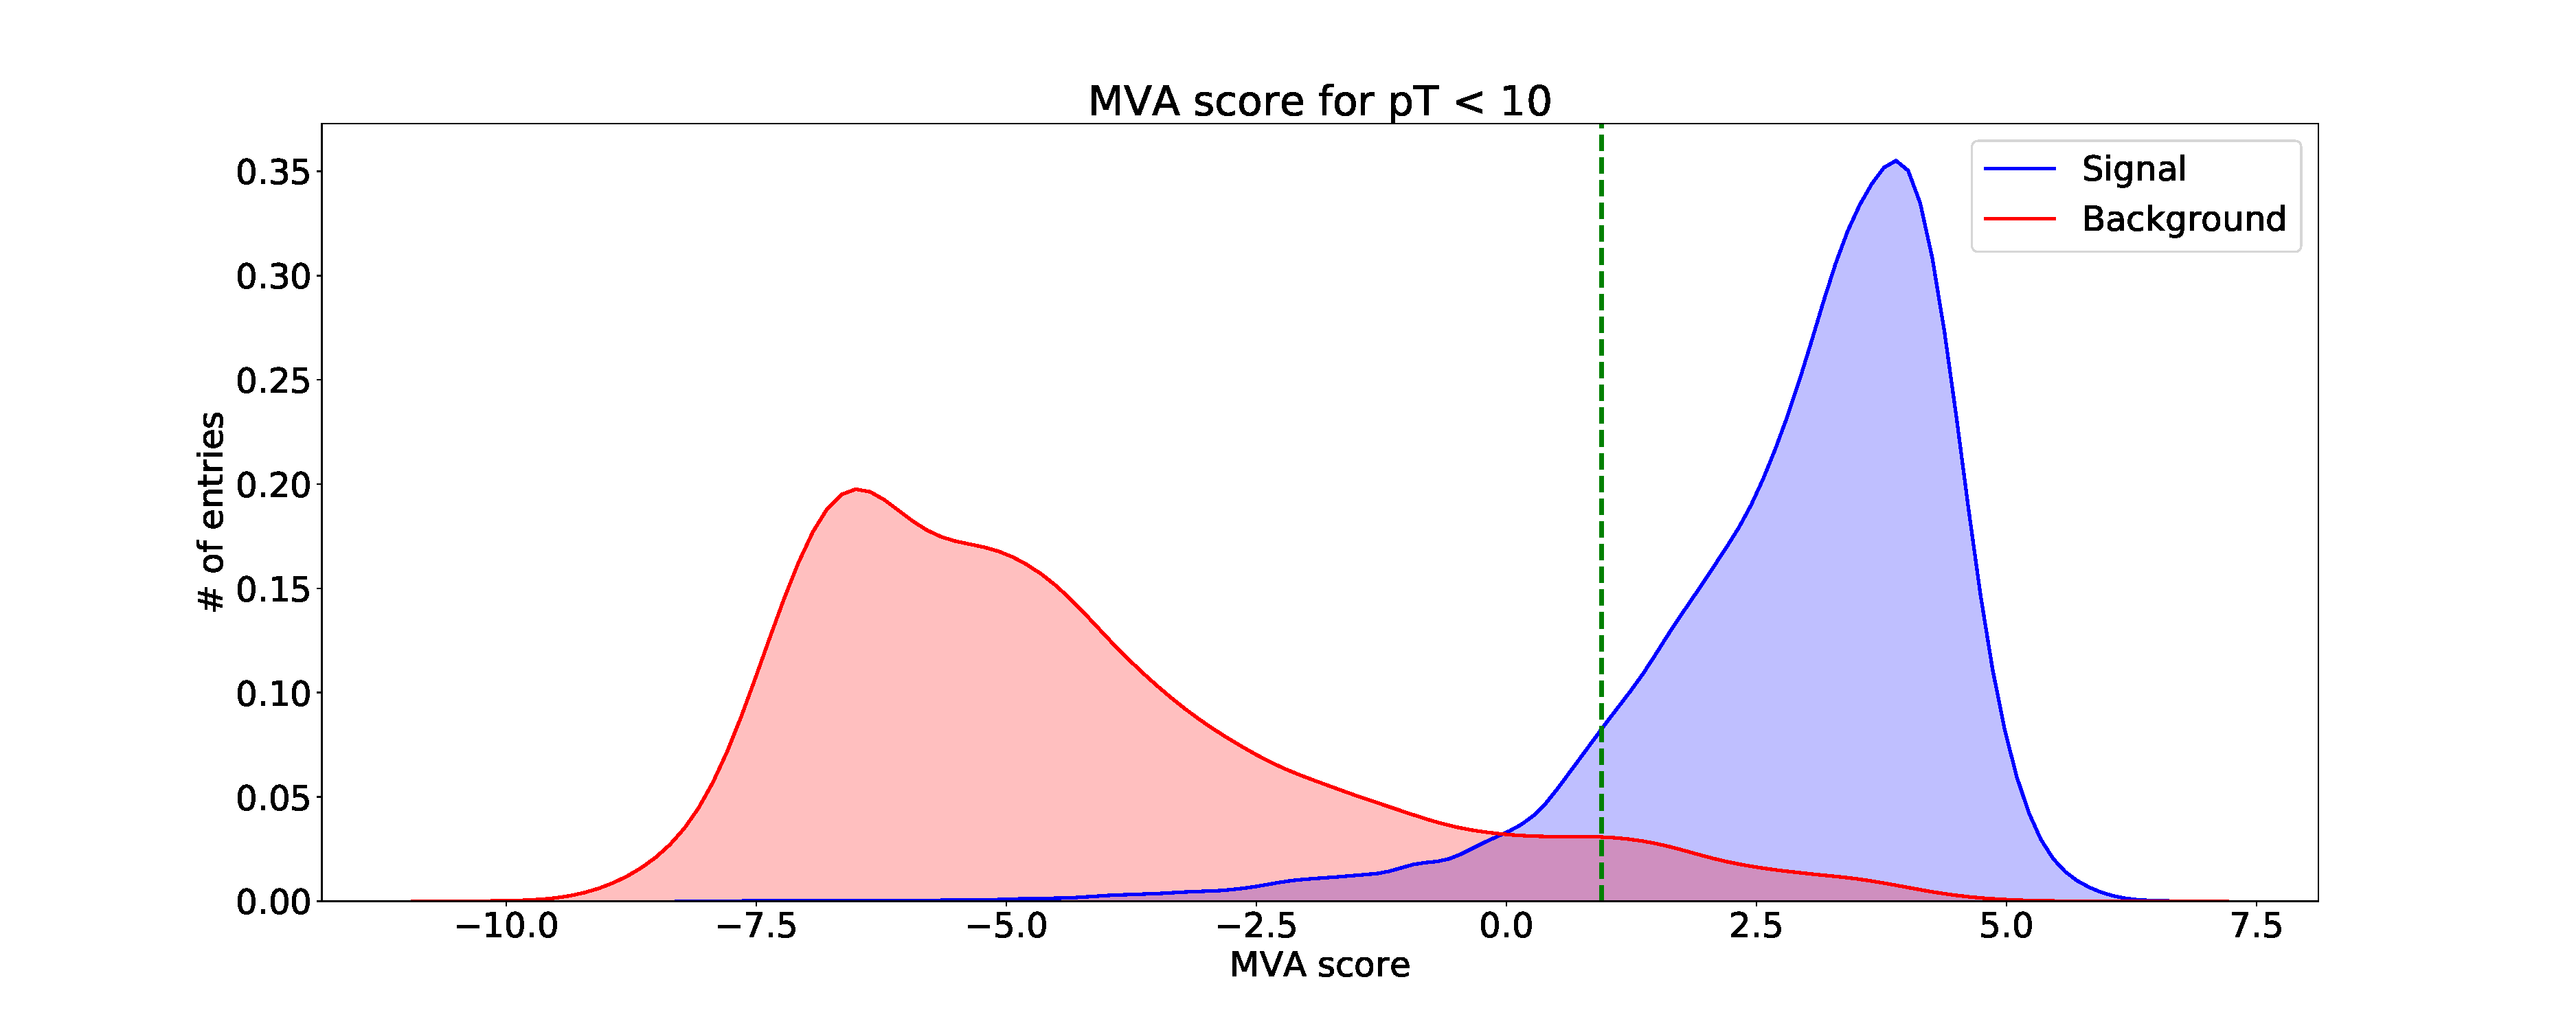
\includegraphics[width=0.95\textwidth]{Figures/Muons/MVA_score_5_2018.pdf}\\
      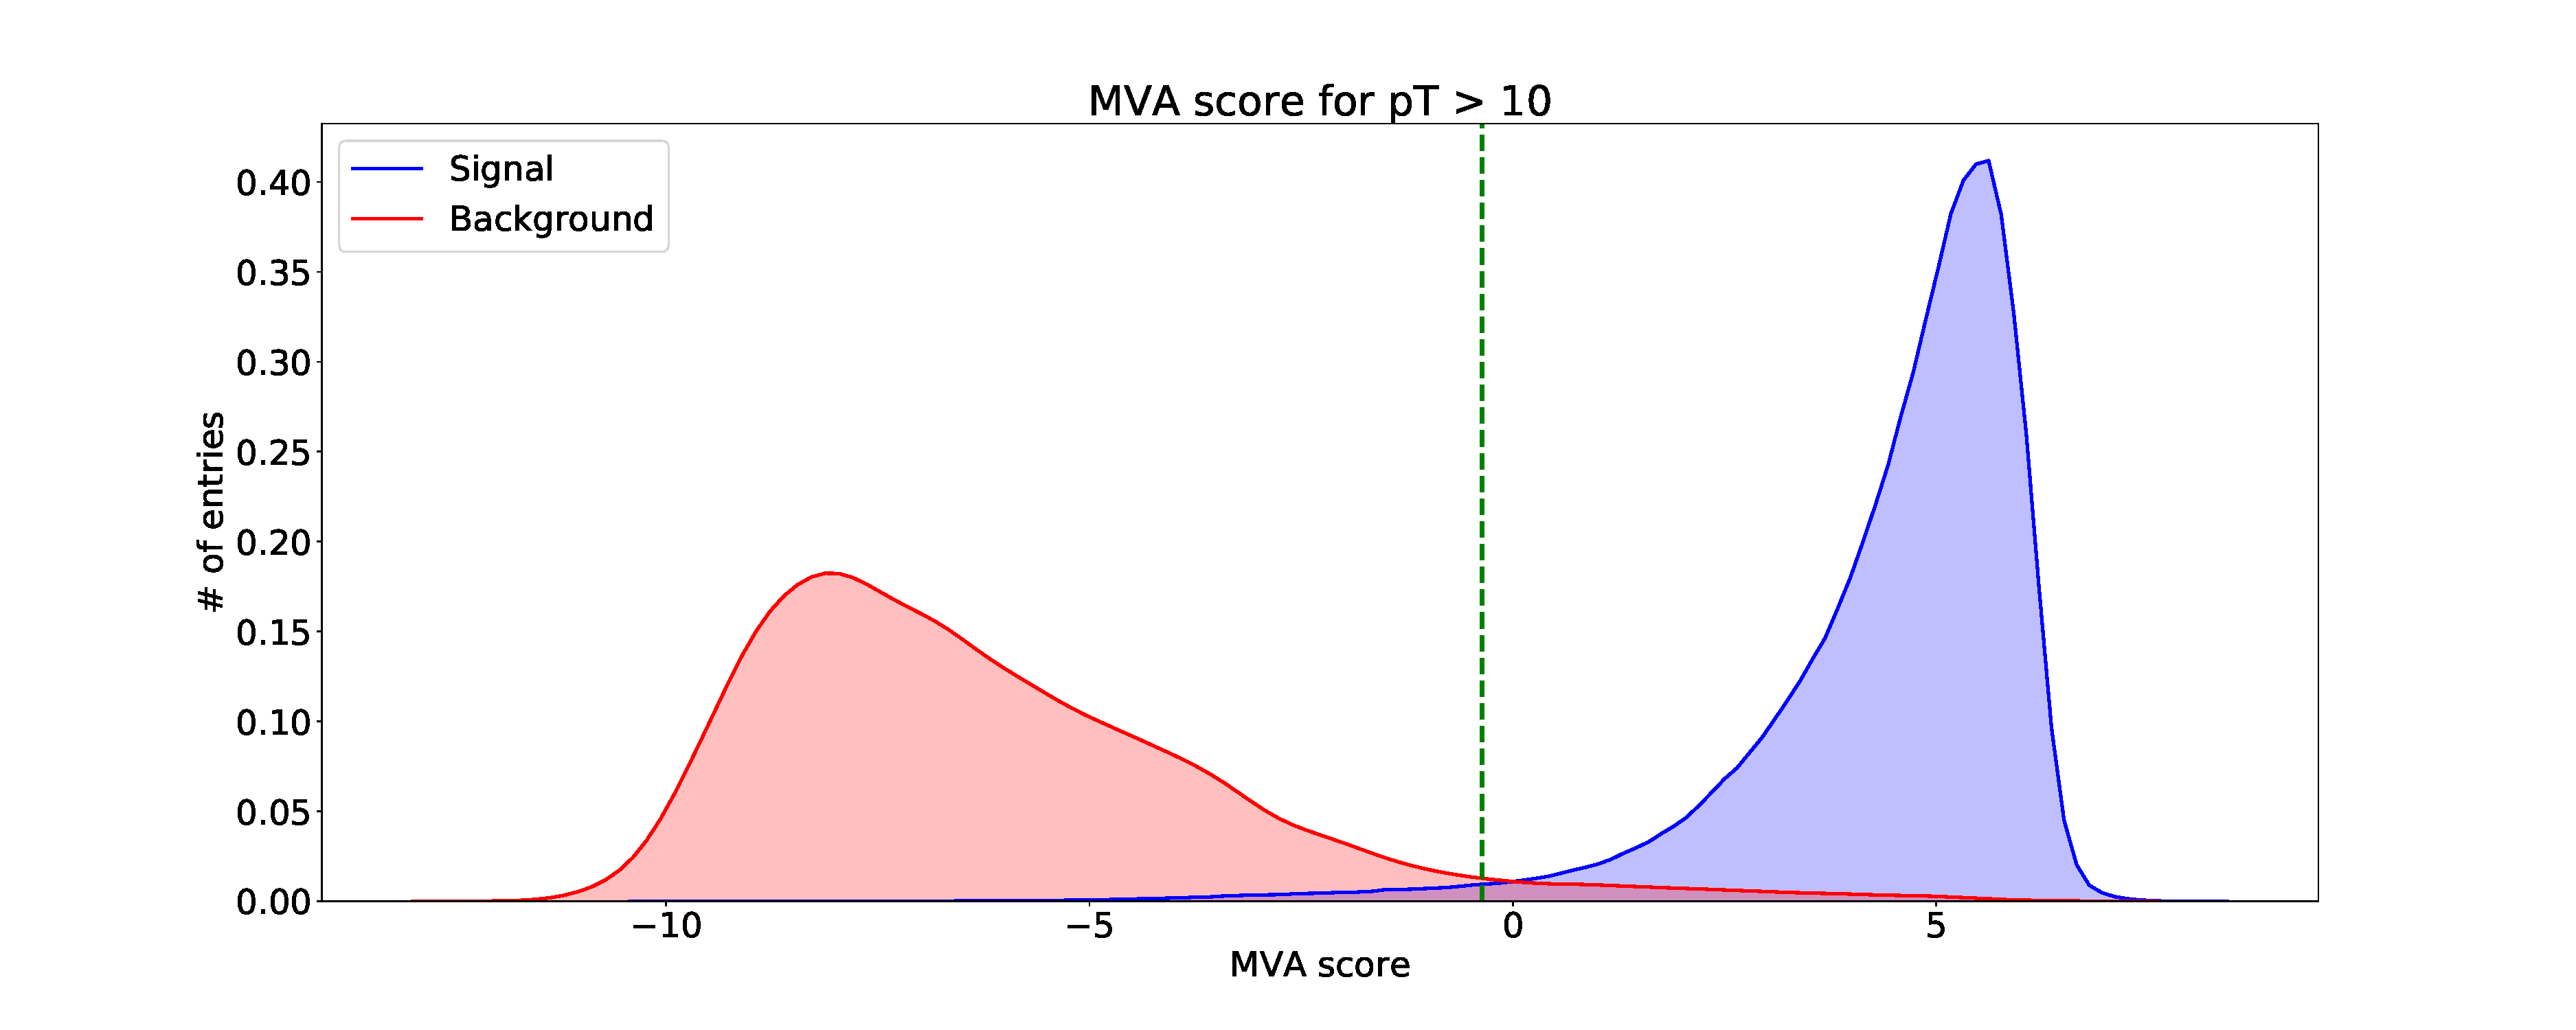
\includegraphics[width=0.95\textwidth]{Figures/Muons/MVA_score_10_2018.pdf}
   \caption{The MVA score and Working Point choice for the MVA trained on 2018 Drell-Yan with jets MC sample. The MVA score is shown for muons with
   $5 < p_T < 10 $ GeV (top) and $p_T > 10$ GeV (bottom).}
   \label{fig:mu_MVA_score_2018}
   \end{center}
\end{figure}


In Figs.~\ref{fig:mu_ID_ISO_SIP_ROC} one can compare ROC curve for the model trained on 2016, 2017, and 2018 MC using muon identification, isolation, and impact
parameter features with the sequential PF muon ID $+$ RelPFiso $< 0.35 +$ SIP3D $< 4$ approach marked with dot. Please note that for the comparison reasons the dot has
been moved below the ROC curve in the ration plot so one can easily read the improvement in percentage. As expected, the MVA based approach outperforms the sequential
approach in all data taking periods.

\begin{figure}[!htb]
   \vspace*{0.3cm}
   \begin{center}
      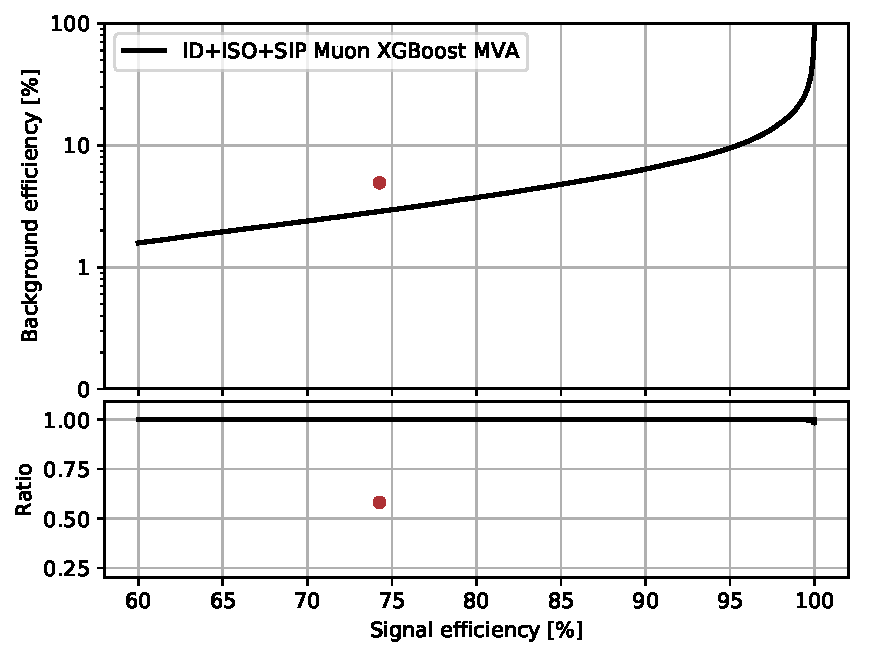
\includegraphics[width=0.45\textwidth]{Figures/Muons/2016_pT_5.pdf}
      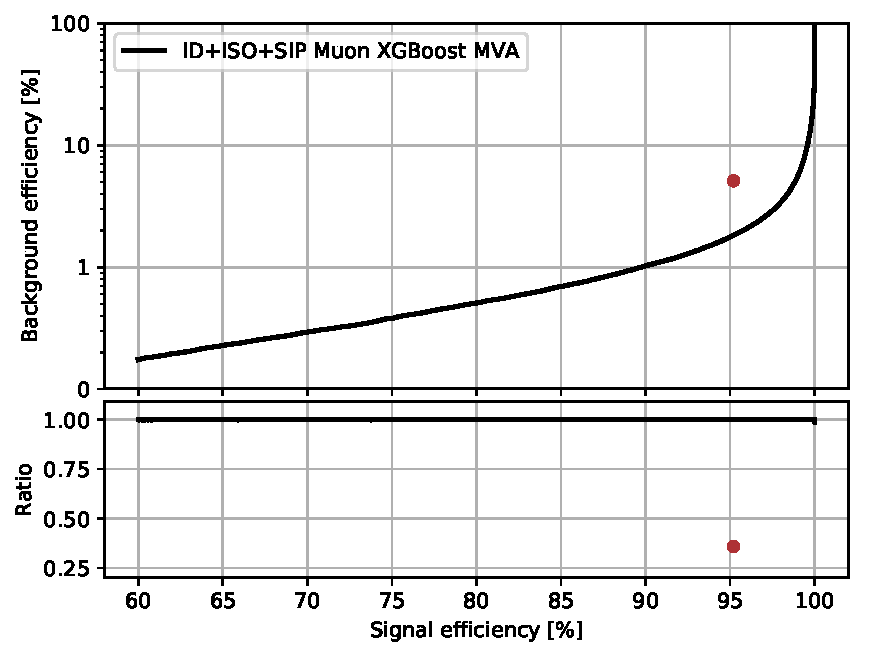
\includegraphics[width=0.45\textwidth]{Figures/Muons/2016_pT_10.pdf} \\
      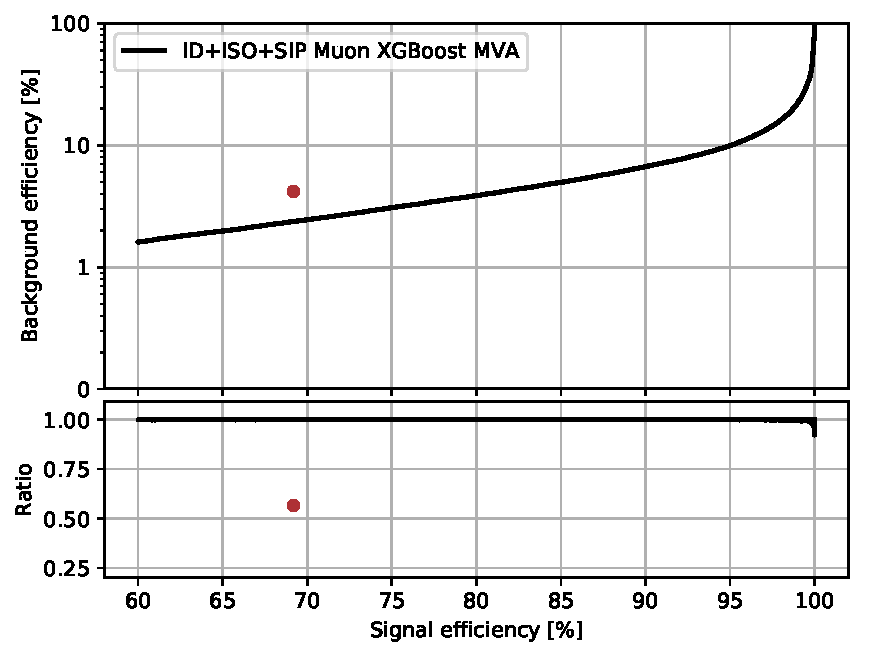
\includegraphics[width=0.45\textwidth]{Figures/Muons/2017_pT_5.pdf}
      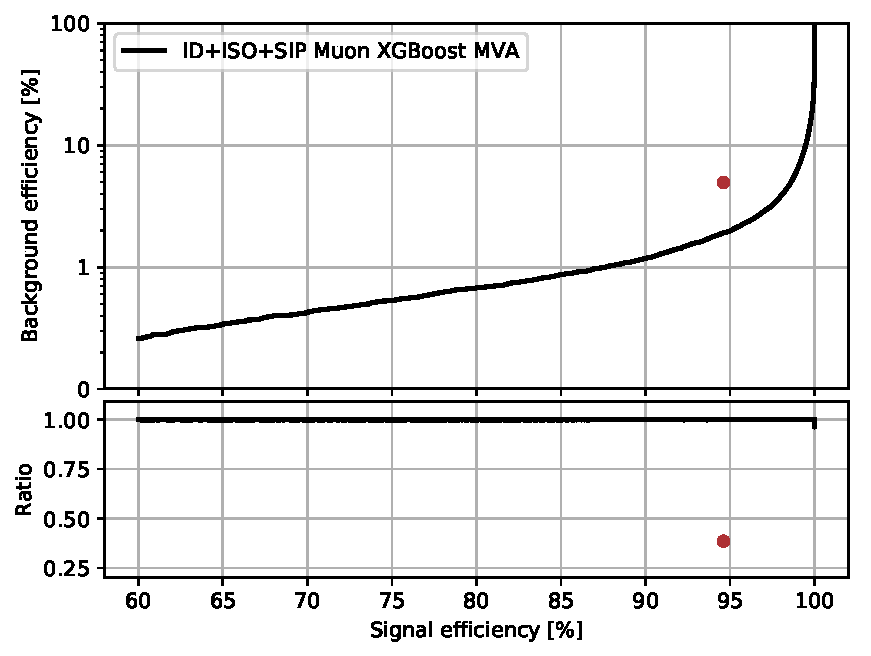
\includegraphics[width=0.45\textwidth]{Figures/Muons/2017_pT_10.pdf} \\
      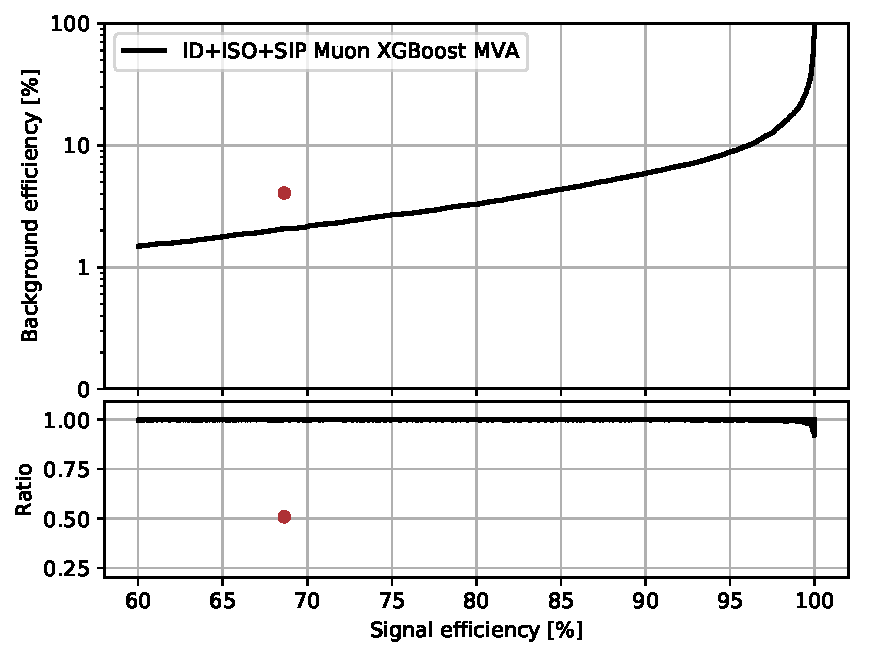
\includegraphics[width=0.45\textwidth]{Figures/Muons/2018_pT_5.pdf}
      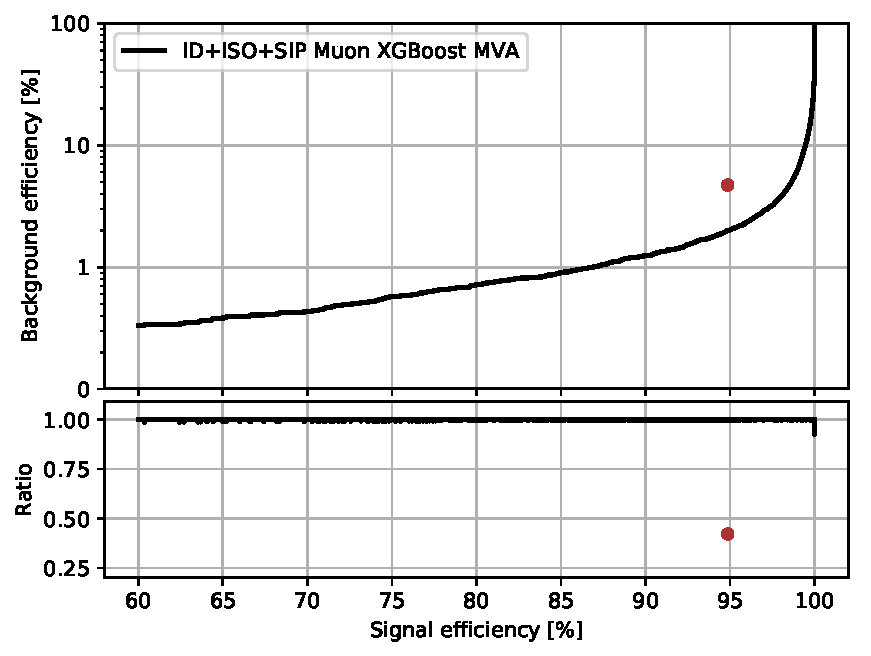
\includegraphics[width=0.45\textwidth]{Figures/Muons/2018_pT_10.pdf} \\
   \caption{The receiver operating characteristic curves, representing the background efficiency vs signal efficiency, of the MVA trained on 2016 (top), 2017
   (middle), and 2018 (bottom) Drell-Yan with jets MC sample. Performance are shown for muons with $5 < p_T < 10 $ GeV (left) and $p_T > 10$ GeV (right) The dot
   represents prevoously used sequential PF muon ID $+$ RelPFiso $< 0.35 +$ SIP3D $< 4$ approach.
   \label{fig:mu_ID_ISO_SIP_ROC}}
   \end{center}
\end{figure}


% Several studies have been conducted on 2016 Drell-Yan with jets MC sample. The XGBoost framework was first used in 2017 and the model was trained on 2017
% Drell-Yan with jets MC sample. This model is known as 2017 ID+ISO V2. The same framework was then used to train the model on 2016 MC (2016 ID+ISO) and finally
% on 2018 MC (2018 ID+ISO). In Fig.~\ref{fig:ele_ID_ISO_ROC_2016} one can see the ROC curves obtained using 2016 Drell-Yan with jets MC sample. As expected, the
% model trained on 2016 MC using electron identification and isolation features outperforms the model trained on 2016 MC using only identification features and
% the model obtained after applying 2017 ID+ISO V2 training on 2016 Drell-Yan with jets MC sample.
%
% In Fig.~\ref{fig:ele_ID_ISO_ROC_2016_} one can see the ROC curve for the model trained on 2016 MC using electron identification and isolation features and ROC
% curve when applying sequential approach meaning applying isolation cut after cutting on the distribution obtained by training using only identification features.
% As expected, the model obtained using electron identification and isolation features outperforms the sequential approach model.
%
% \begin{figure}[!htb]
%    \vspace*{0.3cm}
%    \begin{center}
%       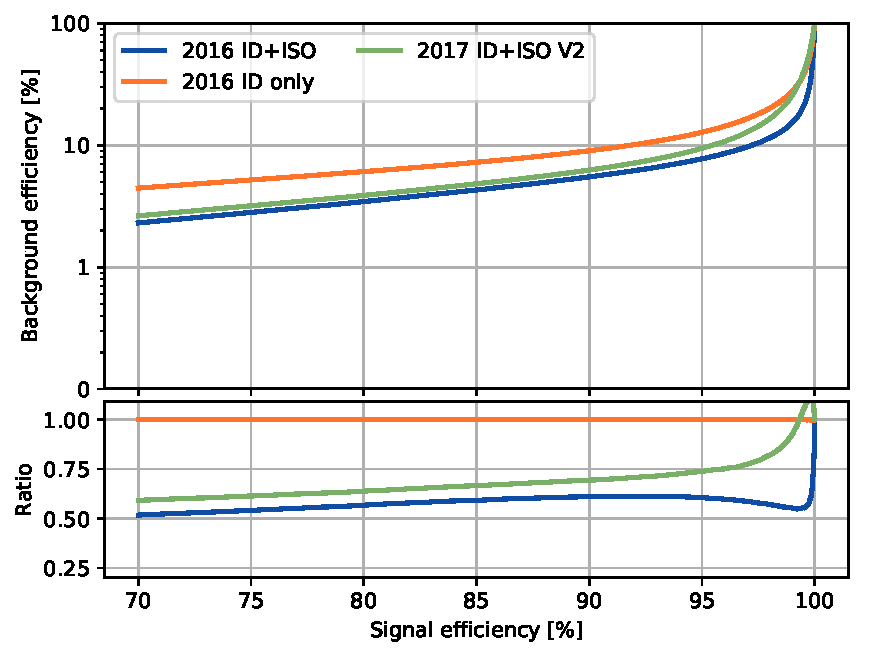
\includegraphics[width=0.45\textwidth]{Figures/Electrons/2016_EB1_5.pdf}
%       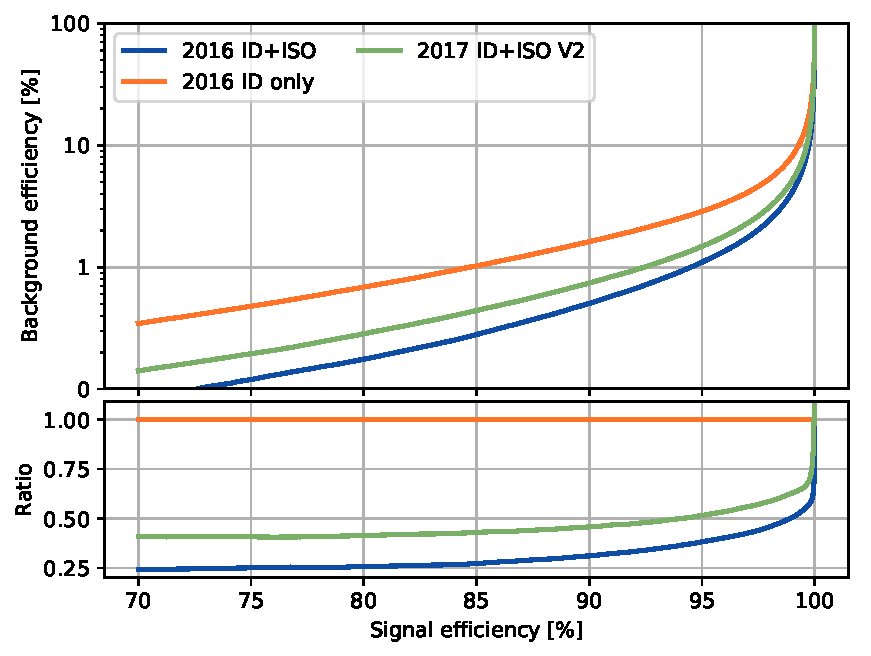
\includegraphics[width=0.45\textwidth]{Figures/Electrons/2016_EB1_10.pdf} \\
%       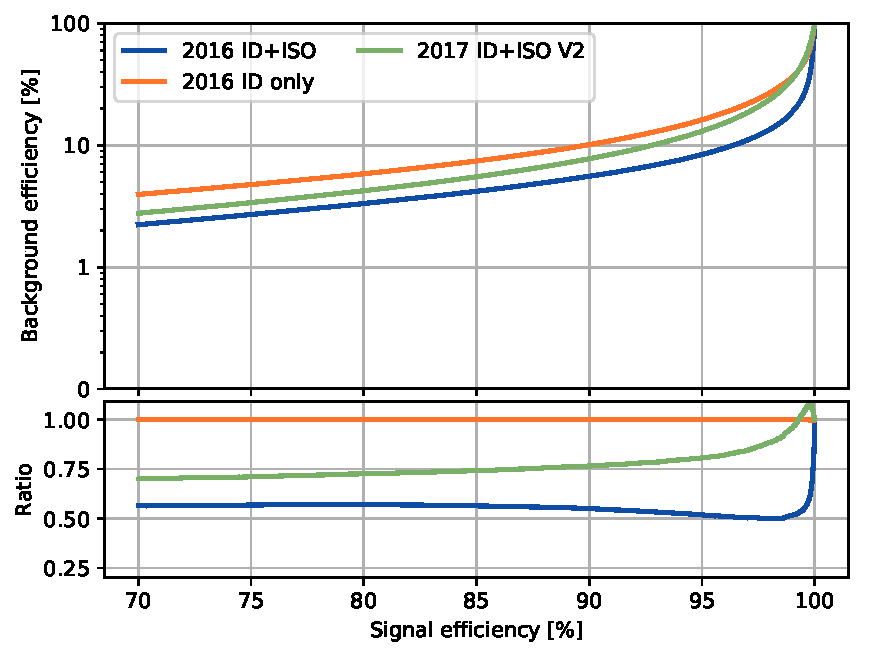
\includegraphics[width=0.45\textwidth]{Figures/Electrons/2016_EB2_5.pdf}
%       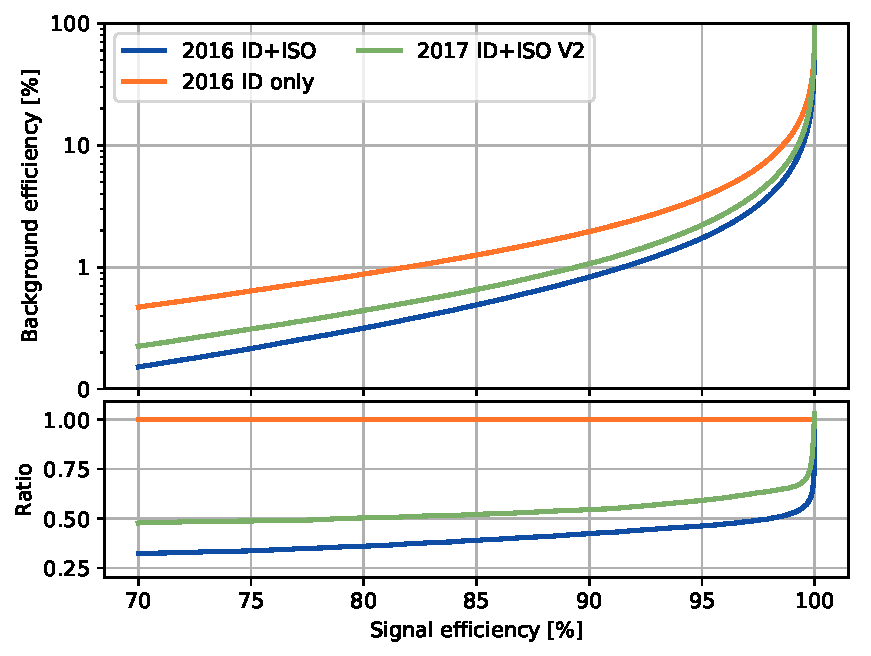
\includegraphics[width=0.45\textwidth]{Figures/Electrons/2016_EB2_10.pdf} \\
%       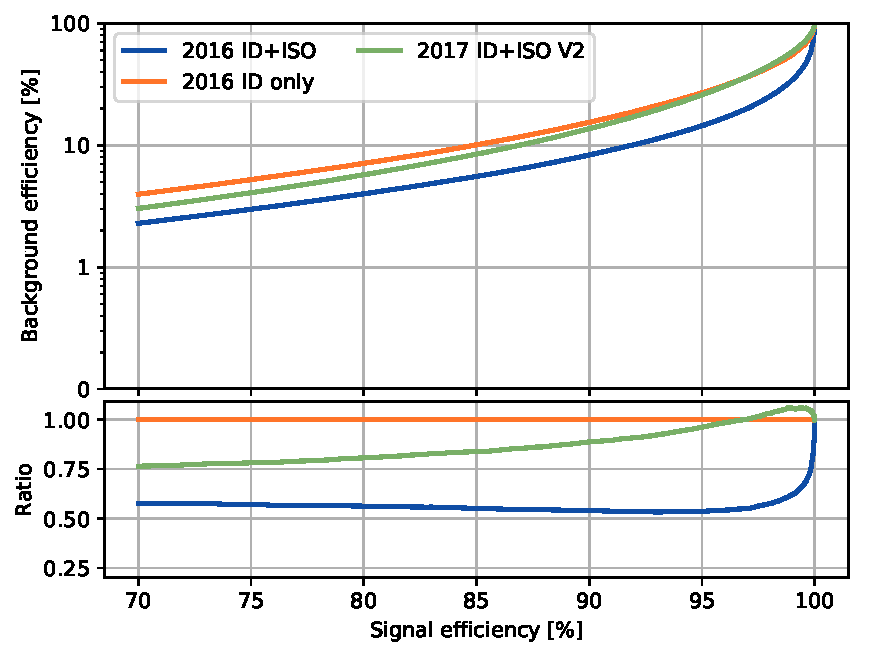
\includegraphics[width=0.45\textwidth]{Figures/Electrons/2016_EE_5.pdf}
%       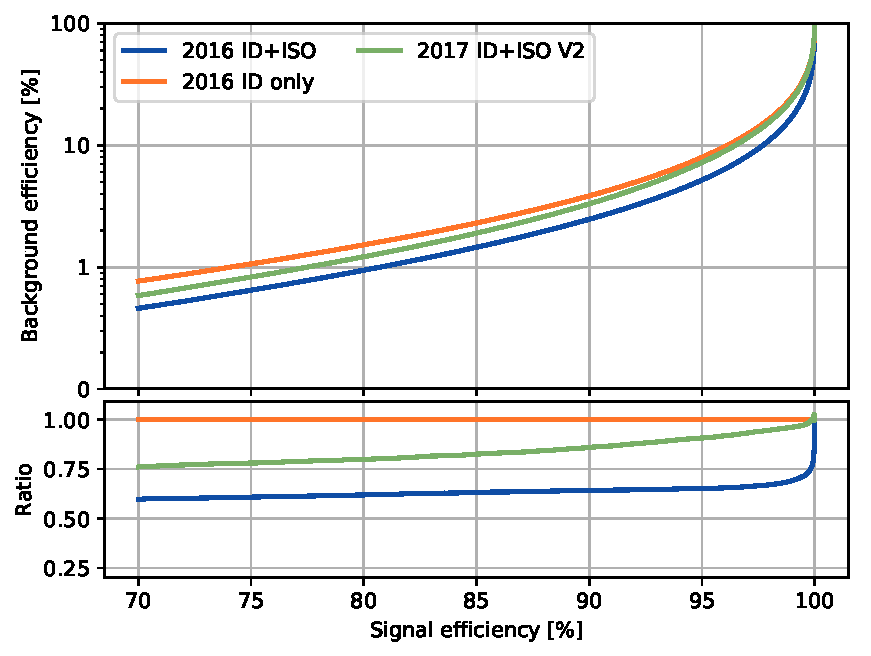
\includegraphics[width=0.45\textwidth]{Figures/Electrons/2016_EE_10.pdf} \\
%    \caption{The receiver operating characteristic curves, representing the background efficiency vs signal efficiency, of the MVA trained on 2016 Drell-Yan with
%    jets MC sample. Performance are shown for electrons with $5 < p_T < 10 $ GeV (left), $p_T > 10$ GeV (right), and $|\eta| < 0.8$ (top),
%    $0.8 < |\eta| < 1.479$ (middle), and $|\eta| > 1.479$ (bottom).
%    \label{fig:ele_ID_ISO_ROC_2016}}
%    \end{center}
% \end{figure}
%
%
% \begin{figure}[!htb]
%    \vspace*{0.3cm}
%    \begin{center}
%       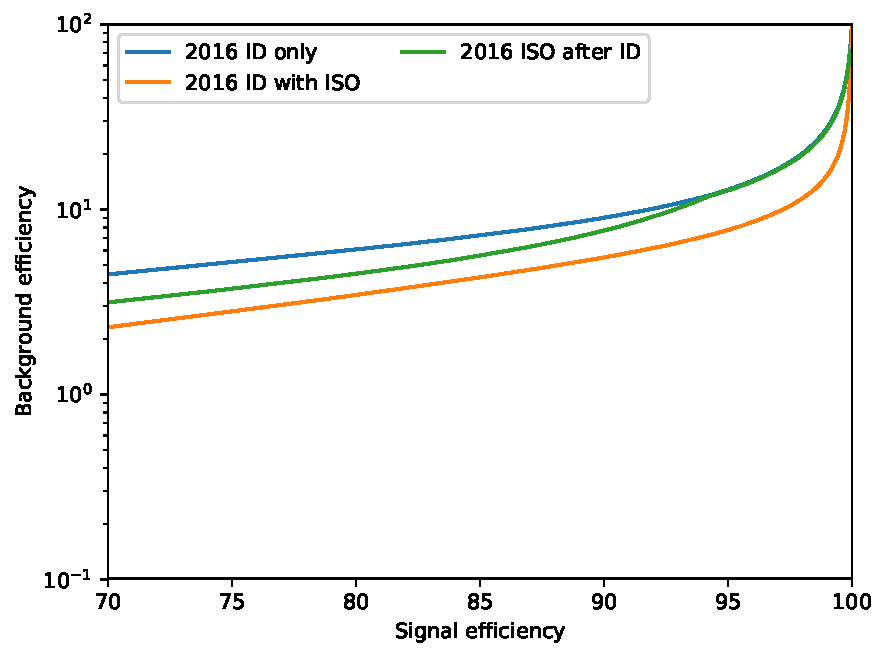
\includegraphics[width=0.45\textwidth]{Figures/Electrons/2016_EB1_5_.pdf}
%       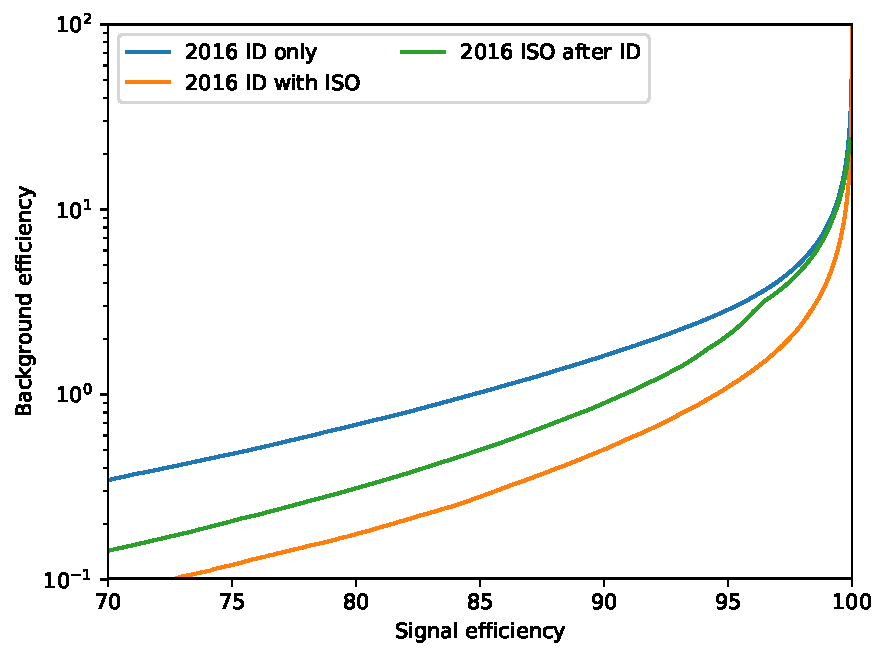
\includegraphics[width=0.45\textwidth]{Figures/Electrons/2016_EB1_10_.pdf} \\
%       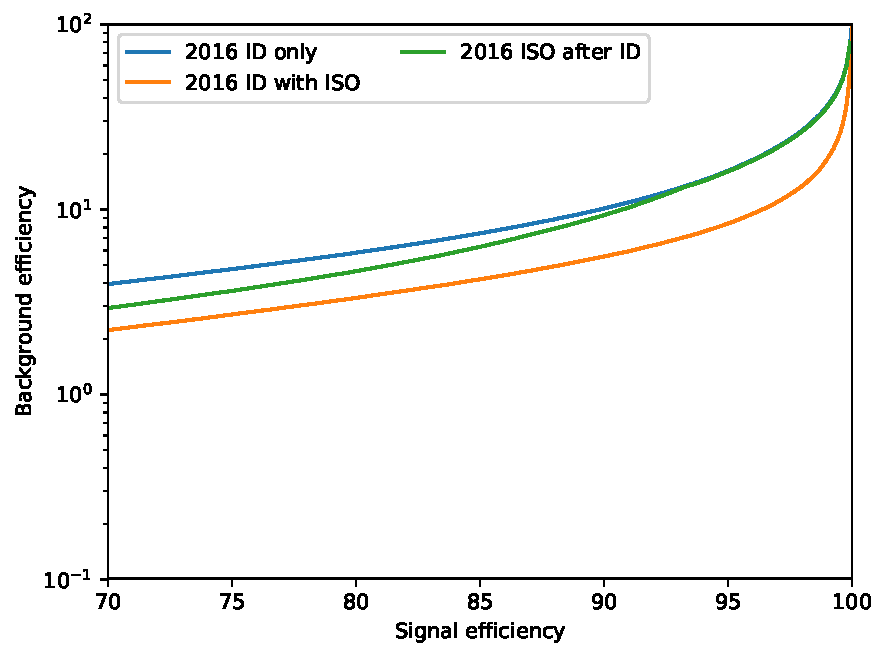
\includegraphics[width=0.45\textwidth]{Figures/Electrons/2016_EB2_5_.pdf}
%       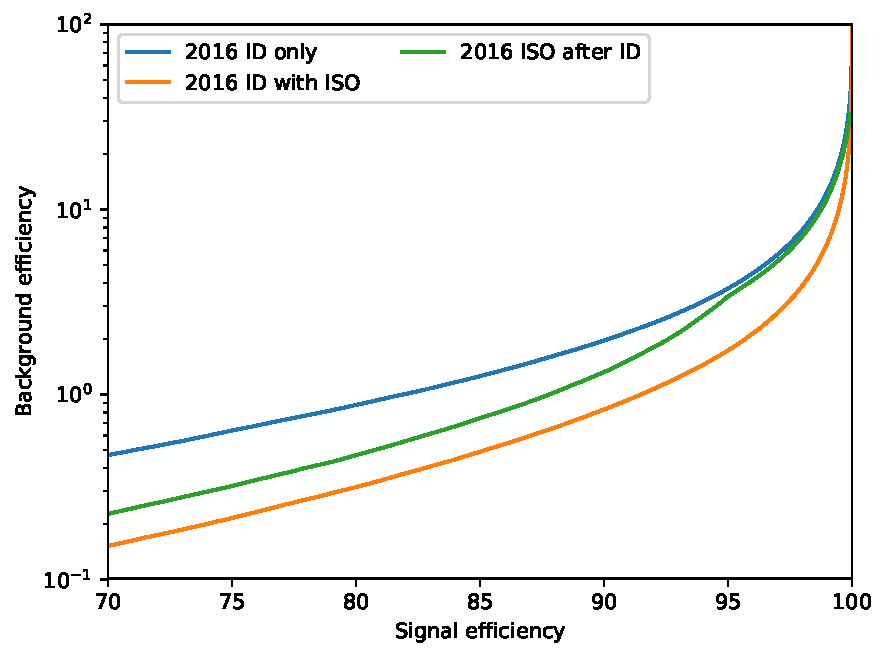
\includegraphics[width=0.45\textwidth]{Figures/Electrons/2016_EB2_10_.pdf} \\
%       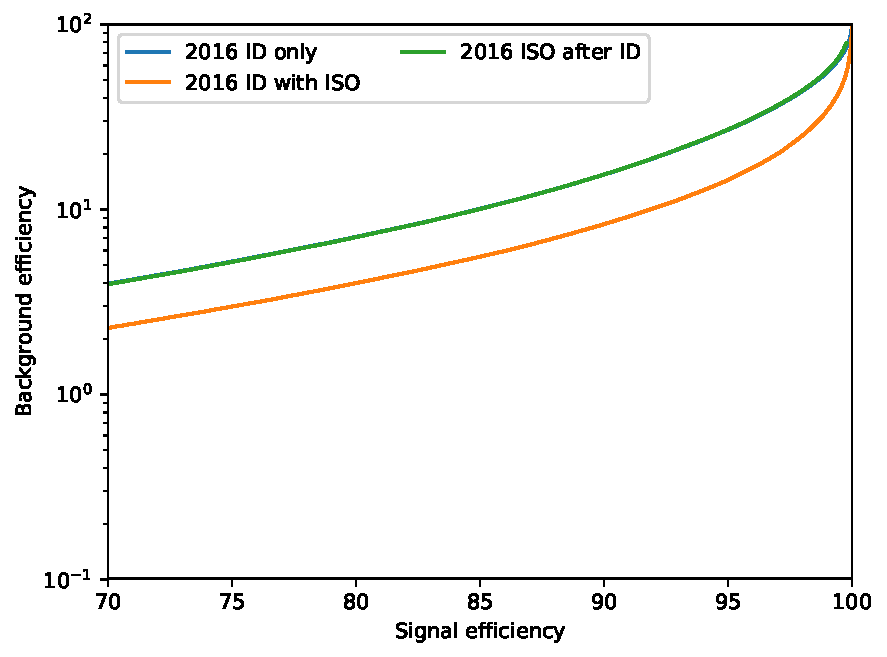
\includegraphics[width=0.45\textwidth]{Figures/Electrons/2016_EE_5_.pdf}
%       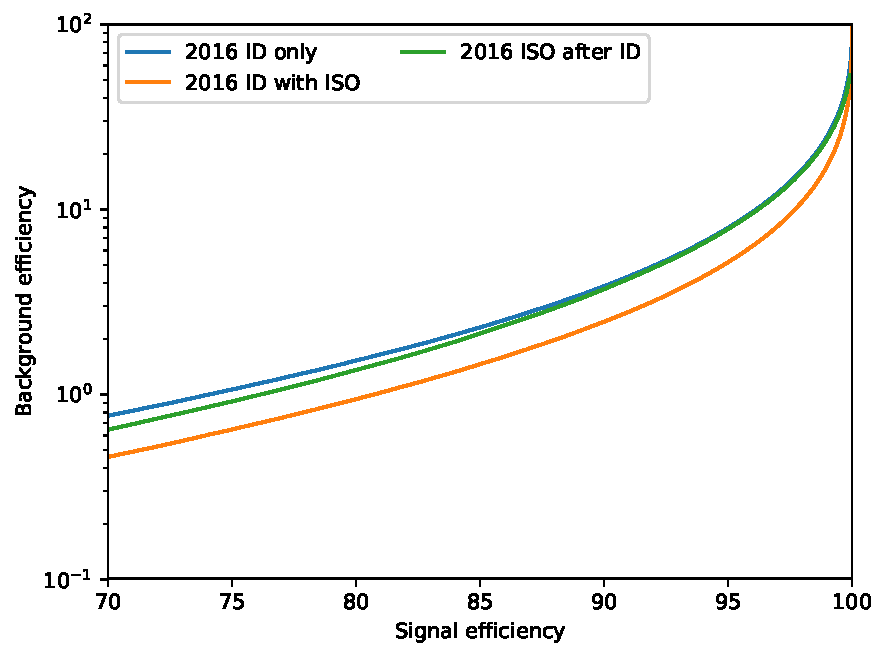
\includegraphics[width=0.45\textwidth]{Figures/Electrons/2016_EE_10_.pdf} \\
%    \caption{The receiver operating characteristic curves, representing the background efficiency vs signal efficiency, of the MVA trained on 2016 Drell-Yan with
%    jets MC sample. Performance are shown for electrons with $5 < p_T < 10 $ GeV (left), $p_T > 10$ GeV (right), and $|\eta| < 0.8$ (top),
%    $0.8 < |\eta| < 1.479$ (middle), and $|\eta| > 1.479$ (bottom).
%    \label{fig:ele_ID_ISO_ROC_2016_}}
%    \end{center}
% \end{figure}
%
% The Fig.~\ref{fig:ele_MVA_score_2018} shows output of the multiclassifier discriminant i.e. MVA score for prompt electrons from Drell-Yan events and
% misindentified electrons originating from jets in Drell-Yan events. The performance of  model trained on 2018 MC using electron identification and isolation
% features outperforms the model obtained after applying 2017 ID+ISO V2 training on 2018 Drell-Yan with jets MC sample as shown in Fig.~\ref{fig:ele_MVA_score_2018}.
%
% \begin{figure}[!htb]
%    \vspace*{0.3cm}
%    \begin{center}
%       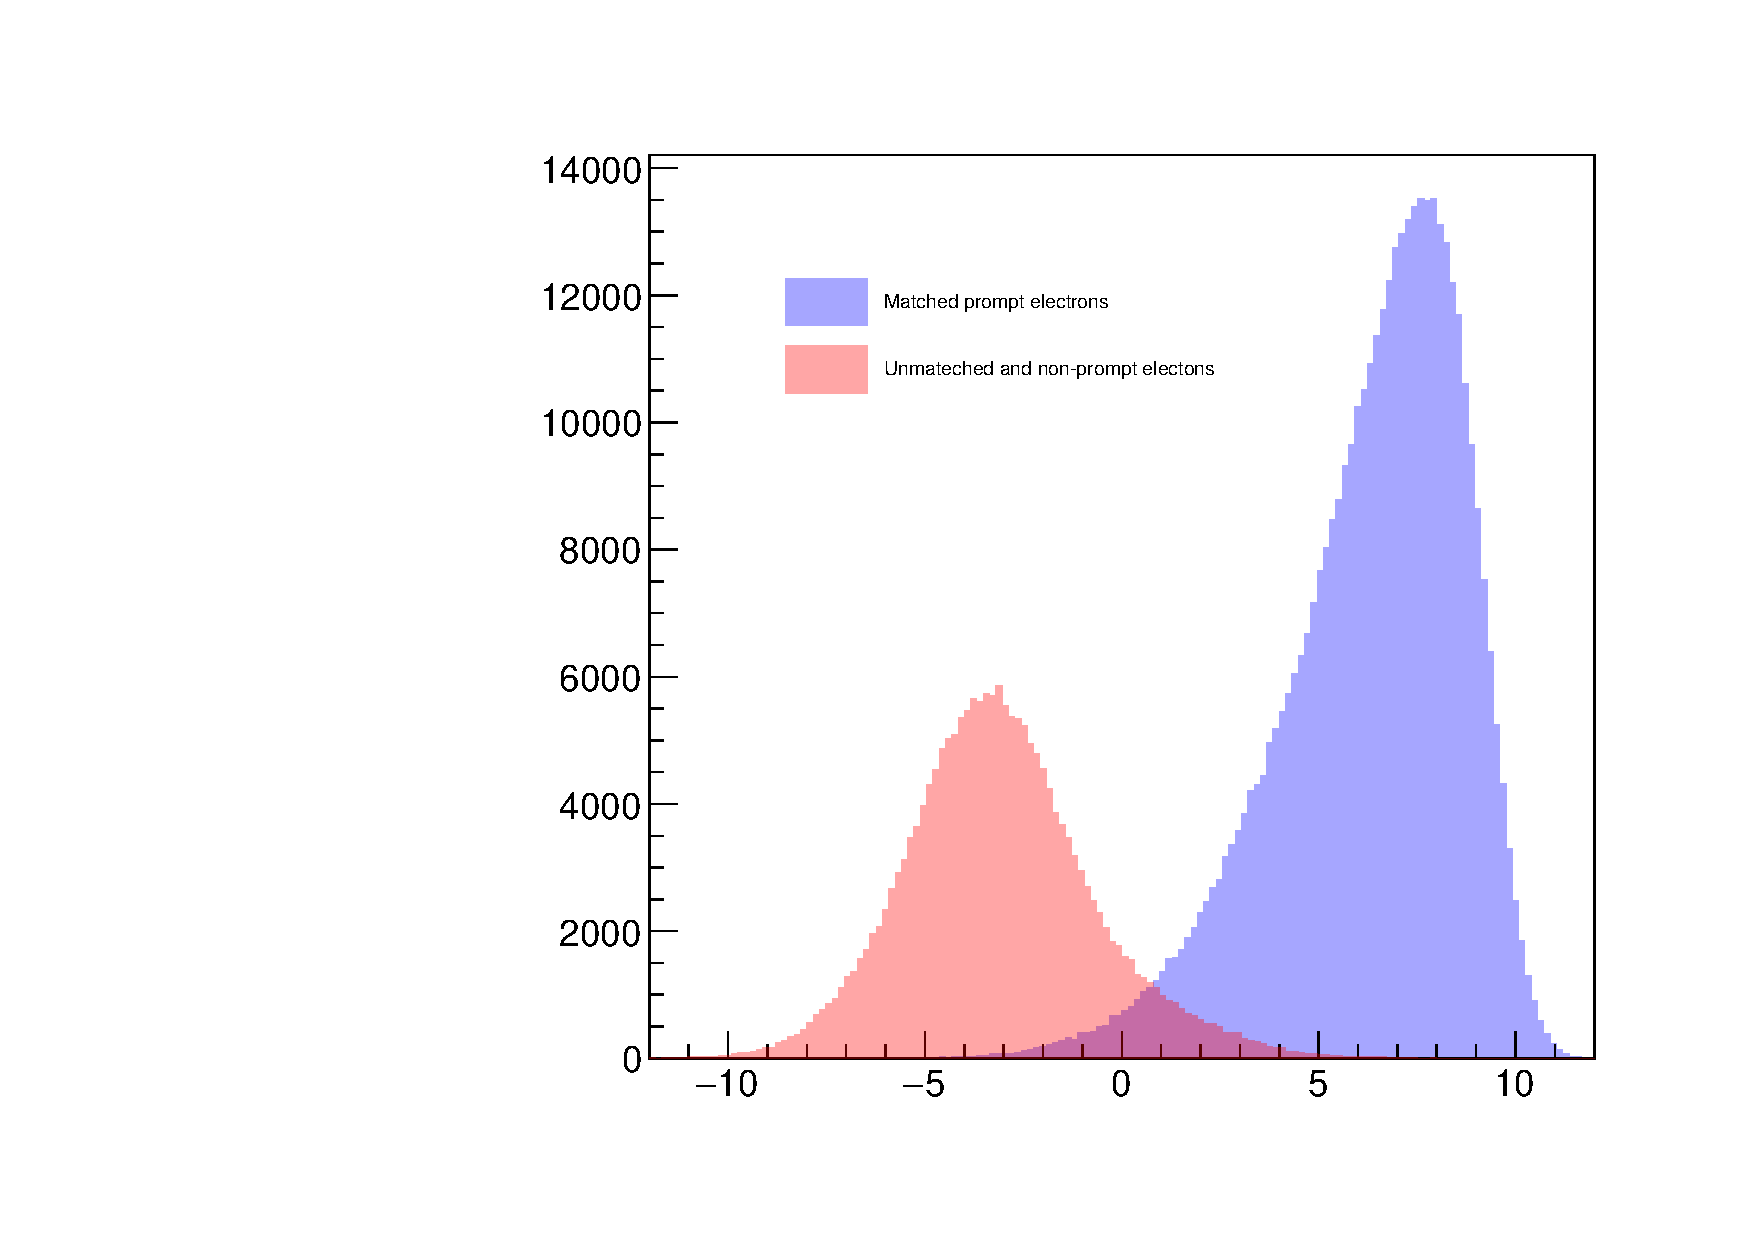
\includegraphics[width=0.80\textwidth]{Figures/Electrons/Ele_BDTv2_Score.pdf}
%       \caption{The Output of the multiclassifier discriminant for prompt electrons matched to truth electrons from $Z$ decay (blue) and for misindentified
%       electrons (red). Events are all taken from Drell-Yan with jets MC sample.
%       \label{fig:ele_MVA_score_2018}}
%    \end{center}
% \end{figure}
%
% \begin{figure}[!htb]
%    \vspace*{0.3cm}
%    \begin{center}
%       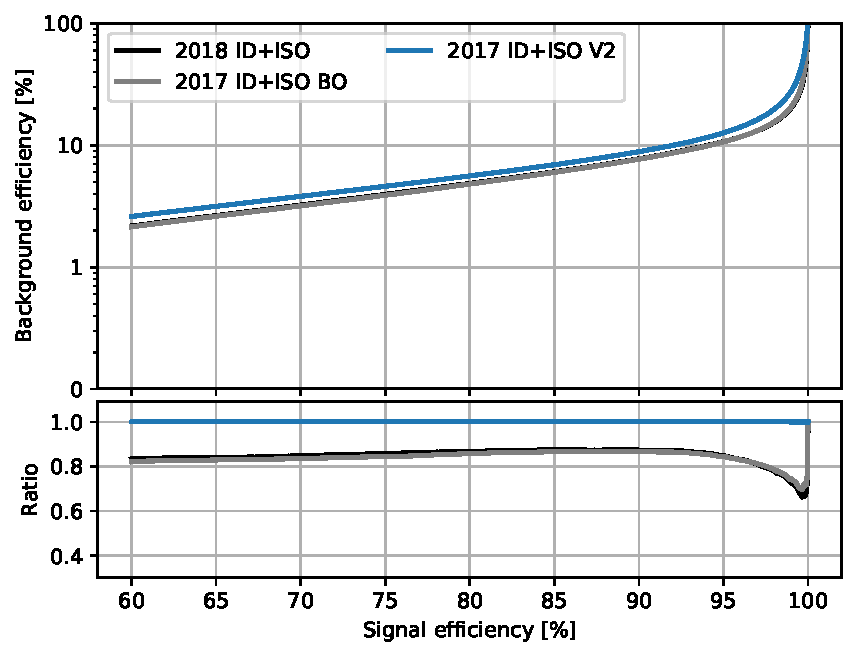
\includegraphics[width=0.45\textwidth]{Figures/Electrons/2018_EB1_5.pdf}
%       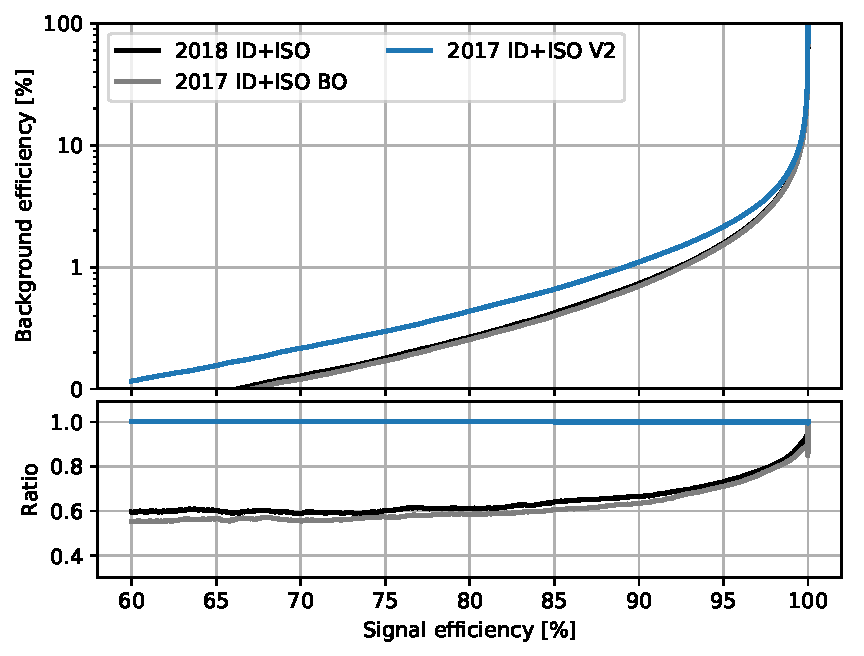
\includegraphics[width=0.45\textwidth]{Figures/Electrons/2018_EB1_10.pdf} \\
%       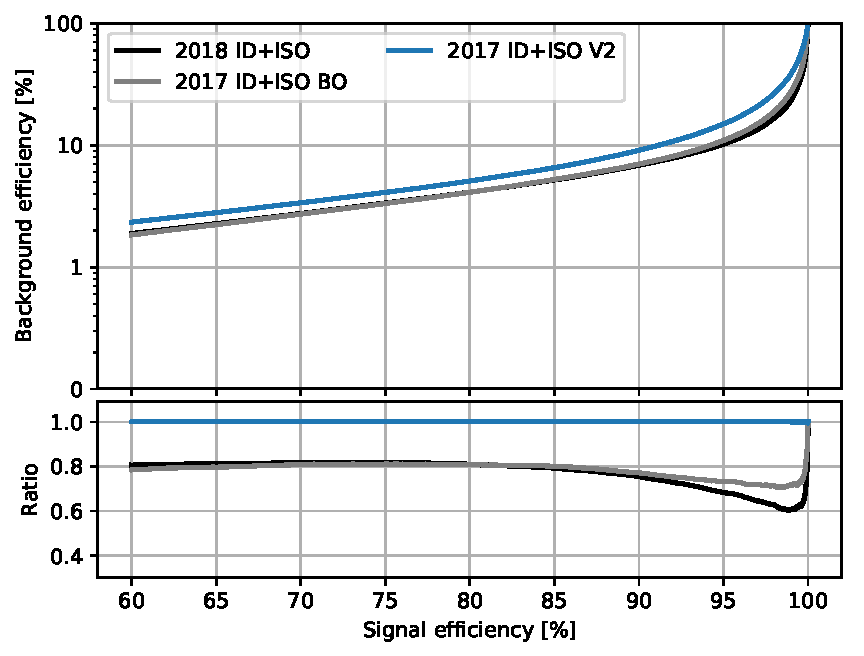
\includegraphics[width=0.45\textwidth]{Figures/Electrons/2018_EB2_5.pdf}
%       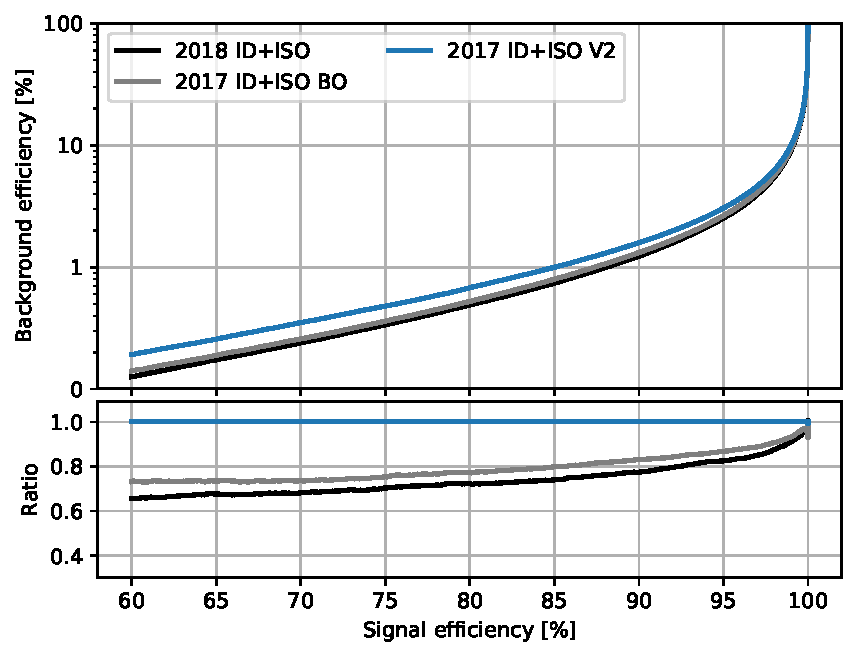
\includegraphics[width=0.45\textwidth]{Figures/Electrons/2018_EB2_10.pdf}\\
%       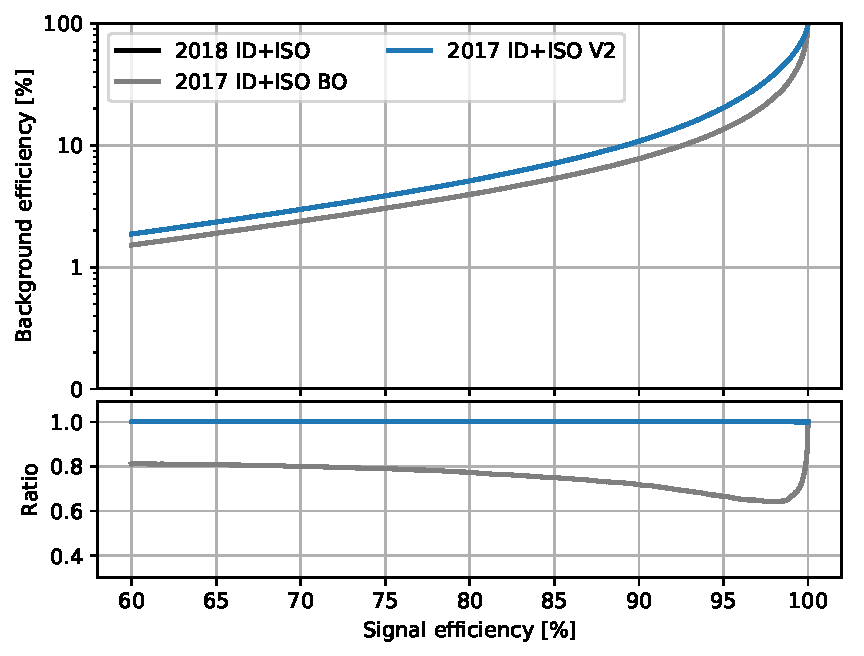
\includegraphics[width=0.45\textwidth]{Figures/Electrons/2018_EE_5.pdf}
%       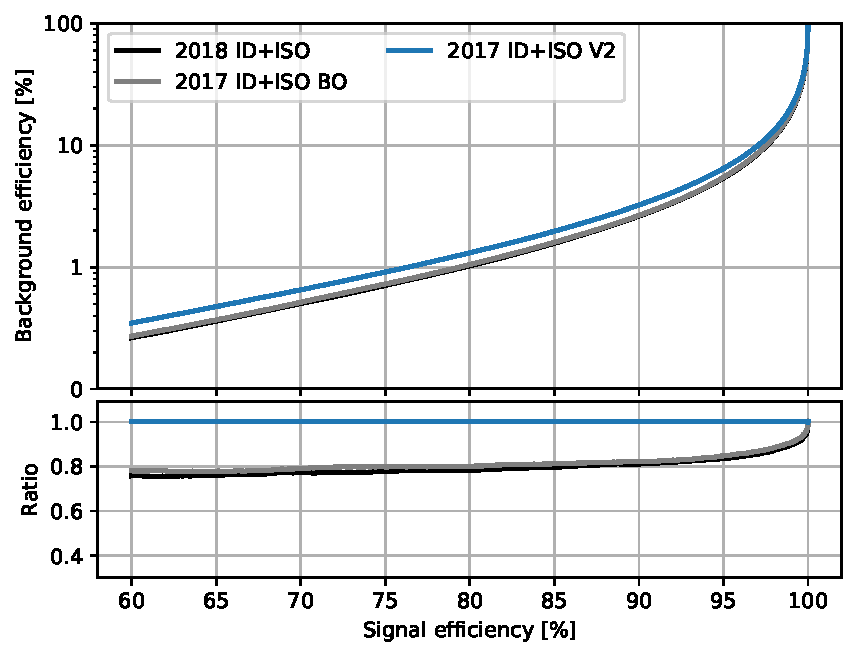
\includegraphics[width=0.45\textwidth]{Figures/Electrons/2018_EE_10.pdf} \\
%    \caption{The receiver operating characteristic curves, representing the background efficiency vs signal efficiency, of the MVA trained on the 2017 Drell-Yan
%    with jets MC sample and applied on the 2018 Drell-Yan with jets MC sample. The training combines identification and isolation fautures. Performance are shown
%    for electrons with $5 < p_T < 10$ GeV (left), $p_T > 10 GeV$ (right), and $|\eta|<0.8$ (top), $0.8 < |\eta| < 1.479$ (middle), and $|\eta| > 1.479$ (bottom).
%    V1 and V2 versions of training are compared, exploiting TMVA and xgboost training libraries respectively.
%    \label{fig:ele_ID_ISO_ROC_2018}}
%    \end{center}
% \end{figure}
%
% The impact of the transition from the TMVA (V1) to the XGBoost(V2) training framework is shown in Fig.~\ref{fig:ele_ID_ISO_ROC_V1_vs_V2}.
% % The working points shown are chosen so as to get the  same signal efficiency as a cut on MVA ID and a cut on the PF isolation, in each $p_T$ and $\eta$ bin.
%
% \begin{figure}[!htb]
%    \vspace*{0.3cm}
%    \begin{center}
%       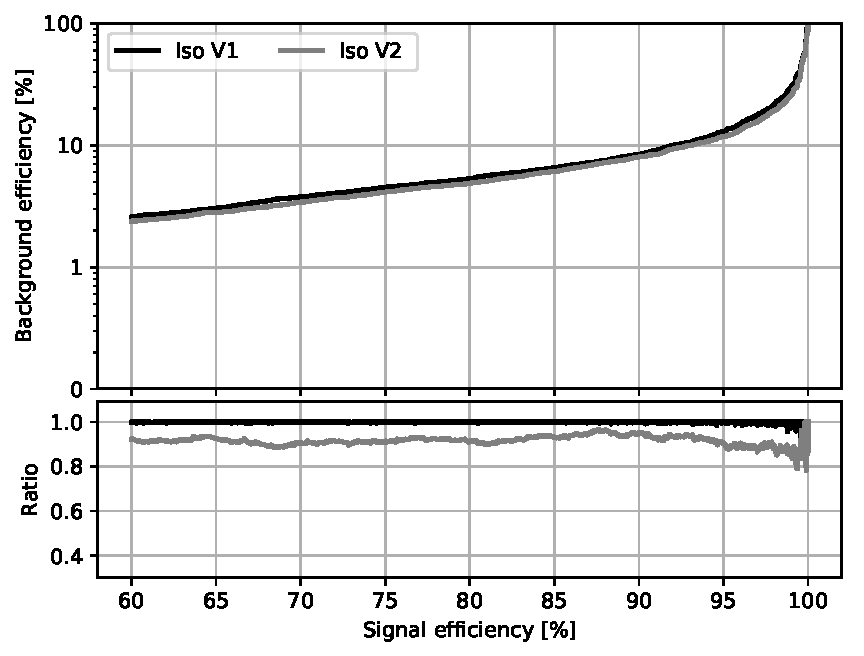
\includegraphics[width=0.45\textwidth]{Figures/Electrons/2018_EB1_5_.pdf}
%       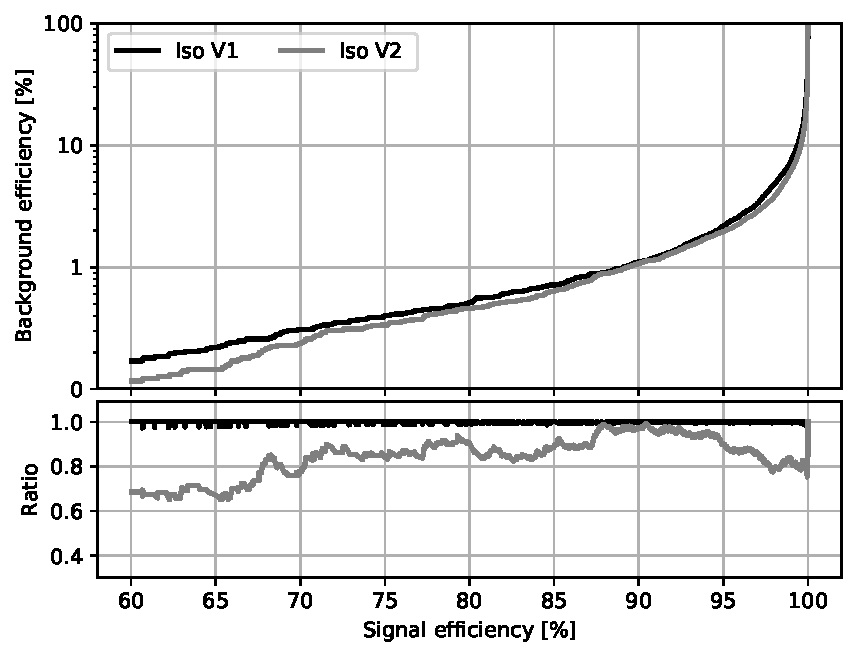
\includegraphics[width=0.45\textwidth]{Figures/Electrons/2018_EB1_10_.pdf} \\
%       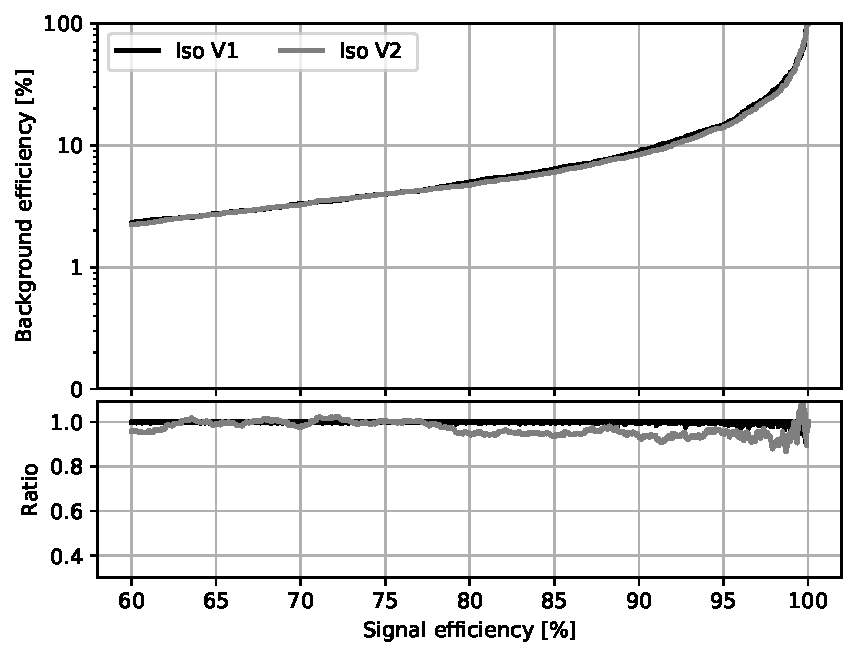
\includegraphics[width=0.45\textwidth]{Figures/Electrons/2018_EB2_5_.pdf}
%       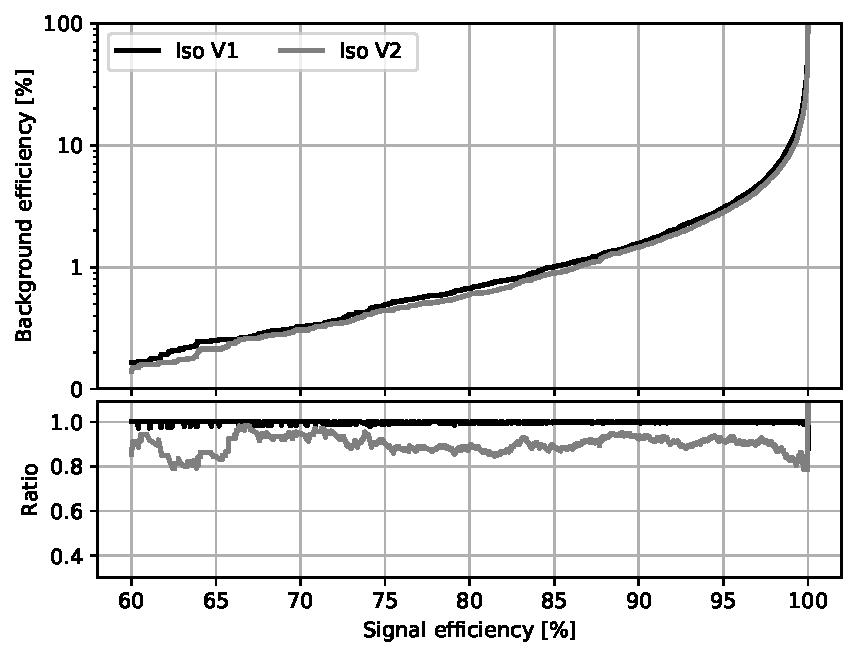
\includegraphics[width=0.45\textwidth]{Figures/Electrons/2018_EB2_10_.pdf} \\
%       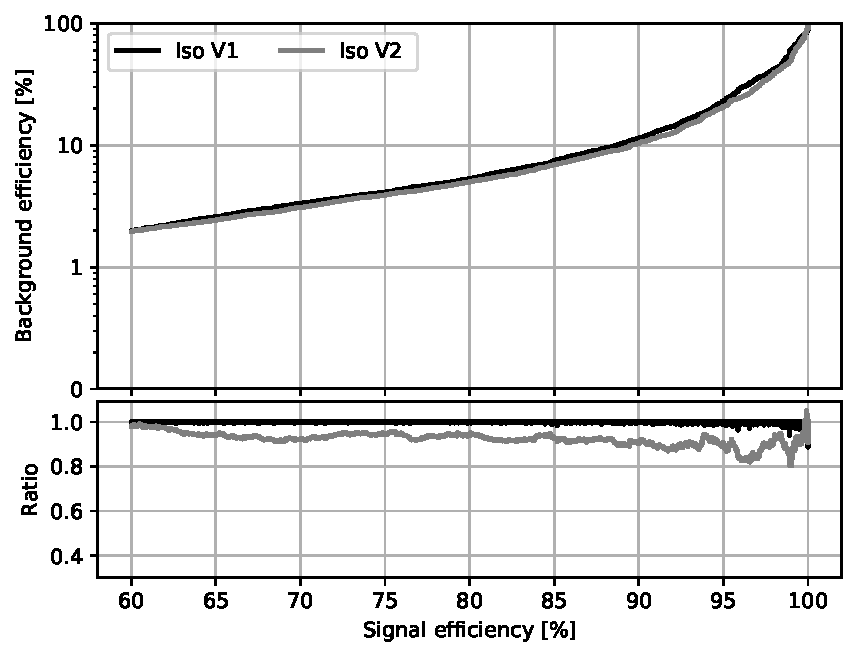
\includegraphics[width=0.45\textwidth]{Figures/Electrons/2018_EE_5_.pdf}
%       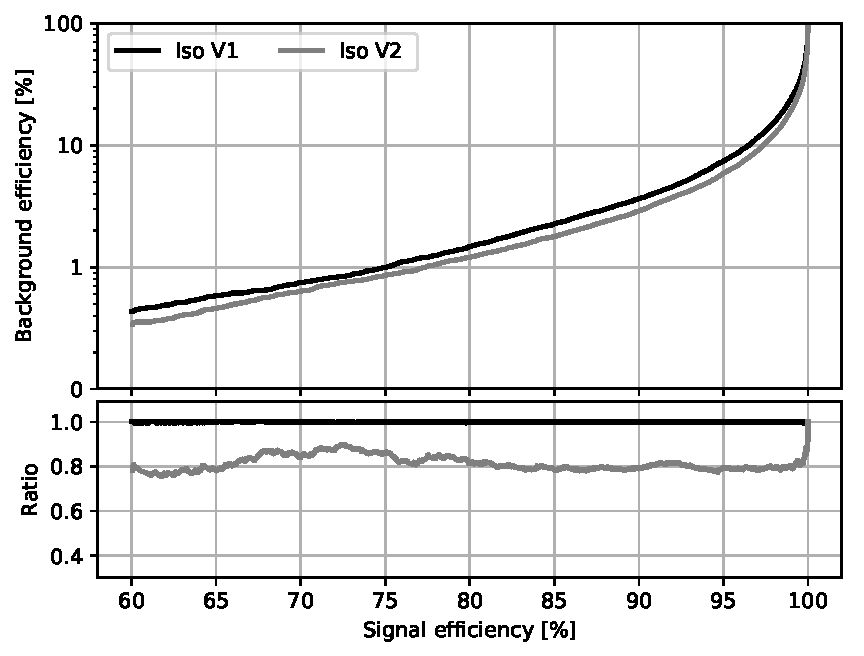
\includegraphics[width=0.45\textwidth]{Figures/Electrons/2018_EE_10_.pdf} \\
%    \caption{Performance comparison, background efficiency vs signal efficiency, of the MVA trained using TMVA framework (V1) and XGBoost framework (V2). The
%    performance are shown for electrons with $5 < p_T < 10$ GeV (left), $p_T > 10 GeV$ (right), and $|\eta|<0.8$ (top), $0.8 < |\eta| < 1.479$ (middle), and
%    $|\eta| > 1.479$ (bottom).
% \label{fig:ele_ID_ISO_ROC_V1_vs_V2}}
% \end{center}
% \end{figure}

Table~\ref{tab:muon_ID_WPA} lists the cuts values applied to the Muon MVA output for 2016, 2017, 2018 trainings.

\begin{table}[h!]
%\scriptsize
    \centering
    \begin{tabular}{|c|c c c|}
%\hline
%\multicolumn{2}{|c|}{2017 Datasets} 
\cline{2-4}
  \multicolumn{1}{ c|}{}             & \multicolumn{3}{|c|}{Minimum BDT score}                        \\
\cline{2-4} %----------------------------------------------------------------------------------------                                                                \\
%\hline %----------------------------------------------------------------------------------------
%minimum BDT score    &  $|\eta| < 0.8 $ & $0.8 < |\eta| < 1.479$ 	& $|\eta| > 1.479$      \\
 \multicolumn{1}{c|}{} & 2016    &  2017 & 2018  \\
\hline %----------------------------------------------------------------------------------------
$ 5 < p_T < 10 $ GeV &  0.8847  & 0.8836   & 0.9506       \\ %   & 0.8268  	& 0.8694		\\
$p_T > 10$ GeV         &  -0.1939 & -0.3831  & -0.3629      \\ %  & 0.9692	& 0.7935	\\
\hline %----------------------------------------------------------------------------------------
%\hline %----------------------------------------------------------------------------------------
     \end{tabular}
\small
    \caption{Minimum BDT score required for passing the muon identification, for 2016, 2017 and 2018 samples.}% \textbf{FIXME: WP to be defined!}}
    \label{tab:muon_ID_WPA}
\end{table}

\clearpage
